%%%%%%%%%%%%%%%%%%%%%%%%%%%%%%%%%%%%%%%%%
% The Legrand Orange Book
% LaTeX Template
% Version 2.4 (26/09/2018)
%
% This template was downloaded from:
% http://www.LaTeXTemplates.com
%
% Original author:
% Mathias Legrand (legrand.mathias@gmail.com) with modifications by:
% Vel (vel@latextemplates.com)
%
% License:
% CC BY-NC-SA 3.0 (http://creativecommons.org/licenses/by-nc-sa/3.0/)
%
% Compiling this template:
% This template uses biber for its bibliography and makeindex for its index.
% When you first open the template, compile it from the command line with the 
% commands below to make sure your LaTeX distribution is configured correctly:
%
% 1) pdflatex main
% 2) makeindex main.idx -s StyleInd.ist
% 3) biber main
% 4) pdflatex main x 2
%
% After this, when you wish to update the bibliography/index use the appropriate
% command above and make sure to compile with pdflatex several times 
% afterwards to propagate your changes to the document.
%
% This template also uses a number of packages which may need to be
% updated to the newest versions for the template to compile. It is strongly
% recommended you update your LaTeX distribution if you have any
% compilation errors.
%
% Important note:
% Chapter heading images should have a 2:1 width:height ratio,
% e.g. 920px width and 460px height.
%
%%%%%%%%%%%%%%%%%%%%%%%%%%%%%%%%%%%%%%%%%

%----------------------------------------------------------------------------------------
%	PACKAGES AND OTHER DOCUMENT CONFIGURATIONS
%----------------------------------------------------------------------------------------

\documentclass[11pt,fleqn,dvipsnames]{book} % Default font size and left-justified equations
\usepackage[dvipsnames]{xcolor}
\usepackage{tikz}
\usepackage{graphicx}
\usetikzlibrary{arrows,automata,positioning,trees,shadows}

\usepackage[font=scriptsize]{caption}
\usepackage{listings}
\usepackage{clrscode3e}
\usepackage[final]{pdfpages}
\usepackage{scrextend}

% Packages to enable extra letters and symbols
\usepackage{upgreek}

%%%%%%%%%%%%%%%%%%%%%%%%%%%%%%%%%%%%%%%%%
% The Legrand Orange Book
% Structural Definitions File
% Version 2.1 (26/09/2018)
%
% Original author:
% Mathias Legrand (legrand.mathias@gmail.com) with modifications by:
% Vel (vel@latextemplates.com)
% 
% This file was downloaded from:
% http://www.LaTeXTemplates.com
%
% License:
% CC BY-NC-SA 3.0 (http://creativecommons.org/licenses/by-nc-sa/3.0/)
%
%%%%%%%%%%%%%%%%%%%%%%%%%%%%%%%%%%%%%%%%%

%----------------------------------------------------------------------------------------
%	VARIOUS REQUIRED PACKAGES AND CONFIGURATIONS
%----------------------------------------------------------------------------------------

\usepackage[dvipsnames]{xcolor} % Required for specifying colors by name

\usepackage{graphicx} % Required for including pictures
\graphicspath{{figures/}} % Specifies the directory where pictures are stored

\usepackage{lipsum} % Inserts dummy text
\usepackage{pifont} % Symbols

\newcommand{\cmark}{\ding{51}}
\newcommand{\xmark}{\ding{55}}

\usepackage{tikz} % Required for drawing custom shapes
\usepackage{tikzpagenodes}
\usetikzlibrary{calc}

\usepackage[english]{babel} % English language/hyphenation

\usepackage{enumitem} % Customize lists
\setlist{nolistsep} % Reduce spacing between bullet points and numbered lists

\usepackage{booktabs} % Required for nicer horizontal rules in tables

\definecolor{ocre}{HTML}{eb9838} % Define the orange color used for highlighting throughout the book
\definecolor{tut}{HTML}{4c9d4c}
\definecolor{good_green}{HTML}{00b294}
\definecolor{bad_red}{HTML}{a80000}
\definecolor{pitfall_orange}{HTML}{ff8c00}

%----------------------------------------------------------------------------------------
%	MARGINS
%----------------------------------------------------------------------------------------

\usepackage{geometry} % Required for adjusting page dimensions and margins

\geometry{
	paper=letterpaper, % Paper size, change to letterpaper for US letter size
	top=3cm, % Top margin
	bottom=3cm, % Bottom margin
	left=3cm, % Left margin
	right=3cm, % Right margin
	headheight=3cm, % Header height
	footskip=1.4cm, % Space from the bottom margin to the baseline of the footer
	headsep=10pt, % Space from the top margin to the baseline of the header
	%showframe, % Uncomment to show how the type block is set on the page
}

%----------------------------------------------------------------------------------------
%	FONTS
%----------------------------------------------------------------------------------------

\usepackage{avant} % Use the Avantgarde font for headings
%\usepackage{times} % Use the Times font for headings
\usepackage{mathptmx} % Use the Adobe Times Roman as the default text font together with math symbols from the Symbol, Chancery and Computer Modern fonts
\DeclareMathAlphabet{\mathcal}{OMS}{cmsy}{m}{n}
\DeclareSymbolFont{symbols}{OMS}{cmsy}{m}{n}
\DeclareSymbolFont{largesymbols}{OMX}{cmex}{m}{n}
\usepackage{microtype} % Slightly tweak font spacing for aesthetics
\usepackage[utf8]{inputenc} % Required for including letters with accents
\usepackage[T1]{fontenc} % Use 8-bit encoding that has 256 glyphs

%----------------------------------------------------------------------------------------
%	BIBLIOGRAPHY AND INDEX
%----------------------------------------------------------------------------------------

\usepackage[style=numeric,citestyle=numeric,sorting=nyt,sortcites=true,autopunct=true,babel=hyphen,hyperref=true,abbreviate=false,backref=true,backend=biber]{biblatex}
\nocite{*}
\addbibresource{bibliography.bib} % BibTeX bibliography file
\defbibheading{bibempty}{}

\usepackage{calc} % For simpler calculation - used for spacing the index letter headings correctly
\usepackage{makeidx} % Required to make an index
\makeindex % Tells LaTeX to create the files required for indexing

%----------------------------------------------------------------------------------------
%	MAIN TABLE OF CONTENTS
%----------------------------------------------------------------------------------------

\usepackage{titletoc} % Required for manipulating the table of contents

\contentsmargin{0cm} % Removes the default margin

% Part text styling (this is mostly taken care of in the PART HEADINGS section of this file)
\titlecontents{part}
	[0cm] % Left indentation
	{\addvspace{20pt}\bfseries} % Spacing and font options for parts
	{}
	{}
	{}

% Chapter text styling
\titlecontents{chapter}
	[1.25cm] % Left indentation
	{\addvspace{12pt}\large\sffamily\bfseries} % Spacing and font options for chapters
	{\color{ocre!60}\contentslabel[\Large\thecontentslabel]{1.25cm}\color{ocre}} % Formatting of numbered sections of this type
	{\color{ocre}} % Formatting of numberless sections of this type
	{\color{ocre!60}\normalsize\;\titlerule*[.5pc]{.}\;\thecontentspage} % Formatting of the filler to the right of the heading and the page number

% Section text styling
\titlecontents{section}
	[1.25cm] % Left indentation
	{\addvspace{3pt}\sffamily\bfseries} % Spacing and font options for sections
	{\contentslabel[\thecontentslabel]{1.25cm}} % Formatting of numbered sections of this type
	{} % Formatting of numberless sections of this type
	{\hfill\color{black}\thecontentspage} % Formatting of the filler to the right of the heading and the page number

% Subsection text styling
\titlecontents{subsection}
	[1.25cm] % Left indentation
	{\addvspace{1pt}\sffamily\small} % Spacing and font options for subsections
	{\contentslabel[\thecontentslabel]{1.25cm}} % Formatting of numbered sections of this type
	{} % Formatting of numberless sections of this type
	{\ \titlerule*[.5pc]{.}\;\thecontentspage} % Formatting of the filler to the right of the heading and the page number

% Figure text styling
\titlecontents{figure}
	[1.25cm] % Left indentation
	{\addvspace{1pt}\sffamily\small} % Spacing and font options for figures
	{\thecontentslabel\hspace*{1em}} % Formatting of numbered sections of this type
	{} % Formatting of numberless sections of this type
	{\ \titlerule*[.5pc]{.}\;\thecontentspage} % Formatting of the filler to the right of the heading and the page number

% Table text styling
\titlecontents{table}
	[1.25cm] % Left indentation
	{\addvspace{1pt}\sffamily\small} % Spacing and font options for tables
	{\thecontentslabel\hspace*{1em}} % Formatting of numbered sections of this type
	{} % Formatting of numberless sections of this type
	{\ \titlerule*[.5pc]{.}\;\thecontentspage} % Formatting of the filler to the right of the heading and the page number

%----------------------------------------------------------------------------------------
%	MINI TABLE OF CONTENTS IN PART HEADS
%----------------------------------------------------------------------------------------

% Chapter text styling
\titlecontents{lchapter}
	[0em] % Left indentation
	{\addvspace{15pt}\large\sffamily\bfseries} % Spacing and font options for chapters
	{\color{ocre}\contentslabel[\Large\thecontentslabel]{1.25cm}\color{ocre}} % Chapter number
	{}  
	{\color{ocre}\normalsize\sffamily\bfseries\;\titlerule*[.5pc]{.}\;\thecontentspage} % Page number

% Section text styling
\titlecontents{lsection}
	[0em] % Left indentation
	{\sffamily\small} % Spacing and font options for sections
	{\contentslabel[\thecontentslabel]{1.25cm}} % Section number
	{}
	{}

% Subsection text styling (note these aren't shown by default, display them by searchings this file for tocdepth and reading the commented text)
\titlecontents{lsubsection}
	[.5em] % Left indentation
	{\sffamily\footnotesize} % Spacing and font options for subsections
	{\contentslabel[\thecontentslabel]{1.25cm}}
	{}
	{}

%----------------------------------------------------------------------------------------
%	HEADERS AND FOOTERS
%----------------------------------------------------------------------------------------

\usepackage{fancyhdr} % Required for header and footer configuration

\pagestyle{fancy} % Enable the custom headers and footers

\renewcommand{\chaptermark}[1]{\markboth{\sffamily\normalsize\bfseries\thechapter.\ #1}{A}} % Styling for the current chapter in the header
\renewcommand{\sectionmark}[1]{\markright{\sffamily\normalsize\thesection\hspace{5pt}#1}{}} % Styling for the current section in the header

\fancyhf{} % Clear default headers and footers

\fancyhead[E]{
    \begin{tikzpicture}[overlay, remember picture]%
        \fill[ocre] (current page.north west) rectangle ($(current page.north east)+(0,-.5in)$);
        \node[anchor=north west, text=white, minimum size=.5in, inner xsep=5mm] at (current page.north west) {\sffamily\normalsize\thepage};
        \node[anchor=north east, text=white, minimum size=.5in, inner xsep=5mm] at (current page.north east) {\leftmark};
    \end{tikzpicture}
}

\fancyhead[O]{
    \begin{tikzpicture}[overlay, remember picture]%
        \fill[ocre] (current page.north west) rectangle ($(current page.north east)+(0,-.5in)$);
        \node[anchor=north east, text=white, minimum size=.5in, inner xsep=5mm] at (current page.north east) {\sffamily\normalsize\thepage};
        \node[anchor=north west, text=white, minimum size=.5in, inner xsep=5mm] at (current page.north west) {\leftmark};
    \end{tikzpicture}
}

%\fancyhead[LE,RO]{\sffamily\normalsize\thepage} % Styling for the page number in the header
%\fancyhead[LO]{\rightmark} % Print the nearest section name on the left side of odd pages
%\fancyhead[RE]{\leftmark} % Print the current chapter name on the right side of even pages
%\fancyfoot[C]{\thepage} % Uncomment to include a footer

\renewcommand{\headrulewidth}{0pt} % Thickness of the rule under the header

\fancypagestyle{plain}{% Style for when a plain pagestyle is specified
	\fancyhead{}\renewcommand{\headrulewidth}{0pt}%
}

% Removes the header from odd empty pages at the end of chapters
\makeatletter
\renewcommand{\cleardoublepage}{
\clearpage\ifodd\c@page\else
\hbox{}
\vspace*{\fill}
\thispagestyle{empty}
\newpage
\fi}

%----------------------------------------------------------------------------------------
%	THEOREM STYLES
%----------------------------------------------------------------------------------------

\usepackage{amsmath,amsfonts,amssymb,amsthm} % For math equations, theorems, symbols, etc

\newcommand{\intoo}[2]{\mathopen{]}#1\,;#2\mathclose{[}}
\newcommand{\ud}{\mathop{\mathrm{{}d}}\mathopen{}}
\newcommand{\intff}[2]{\mathopen{[}#1\,;#2\mathclose{]}}
\renewcommand{\qedsymbol}{$\blacksquare$}
\newtheorem{notation}{Notation}[chapter]

% Boxed/framed environments
\newtheoremstyle{ocrenumbox}% Theorem style name
{0pt}% Space above
{0pt}% Space below
{\normalfont}% Body font
{}% Indent amount
{\small\bf\sffamily\color{ocre}}% Theorem head font
{\;}% Punctuation after theorem head
{0.25em}% Space after theorem head
{\small\sffamily\color{ocre}\thmname{#1}\nobreakspace\thmnumber{\@ifnotempty{#1}{}\@upn{#2}}% Theorem text (e.g. Theorem 2.1)
\thmnote{\nobreakspace\the\thm@notefont\sffamily\bfseries\color{black}---\nobreakspace#3.}} % Optional theorem note

\newtheoremstyle{blacknumex}% Theorem style name
{5pt}% Space above
{5pt}% Space below
{\normalfont}% Body font
{} % Indent amount
{\small\bf\sffamily}% Theorem head font
{\;}% Punctuation after theorem head
{0.25em}% Space after theorem head
{\small\sffamily{\tiny\ensuremath{\blacksquare}}\nobreakspace\thmname{#1}\nobreakspace\thmnumber{\@ifnotempty{#1}{}\@upn{#2}}% Theorem text (e.g. Theorem 2.1)
\thmnote{\nobreakspace\the\thm@notefont\sffamily\bfseries---\nobreakspace#3.}}% Optional theorem note

\newtheoremstyle{blacknumbox} % Theorem style name
{0pt}% Space above
{0pt}% Space below
{\normalfont}% Body font
{}% Indent amount
{\small\bf\sffamily}% Theorem head font
{\;}% Punctuation after theorem head
{0.25em}% Space after theorem head
{\small\sffamily\thmname{#1}\nobreakspace\thmnumber{\@ifnotempty{#1}{}\@upn{#2}}% Theorem text (e.g. Theorem 2.1)
\thmnote{\nobreakspace\the\thm@notefont\sffamily\bfseries---\nobreakspace#3.}}% Optional theorem note

\newtheoremstyle{pinknumbox} % Axiom box style
{0pt}% Space above
{0pt}% Space below
{\normalfont}% Body font
{}% Indent amount
{\small\bf\sffamily}% Theorem head font
{\;}% Punctuation after theorem head
{0.25em}% Space after theorem head
{\small\sffamily\color{magenta}\thmname{#1}\nobreakspace\thmnumber{\@ifnotempty{#1}{}\@upn{#2}}% Theorem text (e.g. Theorem 2.1)
\thmnote{\nobreakspace\the\thm@notefont\sffamily\bfseries---\nobreakspace#3.}}

\newtheoremstyle{greennumbox} % Axiom box style
{0pt}% Space above
{0pt}% Space below
{\normalfont}% Body font
{}% Indent amount
{\small\bf\sffamily}% Theorem head font
{\;}% Punctuation after theorem head
{0.25em}% Space after theorem head
{\small\sffamily\color{Green}\thmname{#1}\nobreakspace\thmnumber{\@ifnotempty{#1}{}\@upn{#2}}% Theorem text (e.g. Theorem 2.1)
\thmnote{\nobreakspace\the\thm@notefont\sffamily\bfseries---\nobreakspace#3.}}

% Non-boxed/non-framed environments
\newtheoremstyle{ocrenum}% Theorem style name
{5pt}% Space above
{5pt}% Space below
{\normalfont}% Body font
{}% Indent amount
{\small\bf\sffamily\color{ocre}}% Theorem head font
{\;}% Punctuation after theorem head
{0.25em}% Space after theorem head
{\small\sffamily\color{ocre}\thmname{#1}\nobreakspace\thmnumber{\@ifnotempty{#1}{}\@upn{#2}}% Theorem text (e.g. Theorem 2.1)
\thmnote{\nobreakspace\the\thm@notefont\sffamily\bfseries\color{black}---\nobreakspace#3.}} % Optional theorem note
\makeatother

% Defines the theorem text style for each type of theorem to one of the three styles above
\newcounter{dummy} 
\numberwithin{dummy}{section}
\theoremstyle{ocrenumbox}
\newtheorem{theoremeT}[dummy]{Theorem}
\newtheorem{problem}{Problem}[chapter]
\newtheorem{exerciseT}{Exercise}[chapter]
\theoremstyle{blacknumex}
\newtheorem{exampleT}{Example}[chapter]
\theoremstyle{blacknumbox}
\newtheorem{vocabulary}{Vocabulary}[chapter]
\newtheorem{definitionT}{Definition}[section]
\newtheorem{corollaryT}[dummy]{Corollary}
\newtheorem{lemmaT}[dummy]{Lemma}
\theoremstyle{ocrenum}
\newtheorem{proposition}[dummy]{Proposition}
\theoremstyle{pinknumbox}
\newtheorem{axiomT}[dummy]{Axiom}
\theoremstyle{greennumbox}
\newtheorem{ruleT}{Template}[chapter]

% A new set of theorem definitions used in appendix only
\newcounter{appendixcounter}
\theoremstyle{greennumbox}
\newtheorem{ruleT_appendix}[appendixcounter]{Template}
\theoremstyle{pinknumbox}
\newtheorem{axiomT_appendix}[appendixcounter]{Axiom}
\theoremstyle{ocrenumbox}
\newtheorem{theoremeT_appendix}[appendixcounter]{Theorem}

%----------------------------------------------------------------------------------------
%	DEFINITION OF COLORED BOXES
%----------------------------------------------------------------------------------------

\RequirePackage[framemethod=default]{mdframed} % Required for creating the theorem, definition, exercise and corollary boxes

% Theorem box
\newmdenv[skipabove=1em,
skipbelow=7pt,
backgroundcolor=black!5,
linecolor=ocre,
innerleftmargin=5pt,
innerrightmargin=5pt,
innertopmargin=1.5em,
leftmargin=0cm,
rightmargin=0cm,
innerbottommargin=5pt]{tBox}

% Exercise box	  
\newmdenv[skipabove=1em,
skipbelow=7pt,
rightline=false,
leftline=true,
topline=false,
bottomline=false,
backgroundcolor=ocre!10,
linecolor=ocre,
innerleftmargin=5pt,
innerrightmargin=5pt,
innertopmargin=1em,
innerbottommargin=5pt,
leftmargin=0cm,
rightmargin=0cm,
linewidth=4pt]{eBox}	

% Definition box
\newmdenv[skipabove=1em,
skipbelow=7pt,
rightline=false,
leftline=true,
topline=false,
bottomline=false,
linecolor=ocre,
innerleftmargin=5pt,
innerrightmargin=5pt,
innertopmargin=1em,
leftmargin=0cm,
rightmargin=0cm,
linewidth=4pt,
innerbottommargin=0pt]{dBox}	

% Corollary box
\newmdenv[skipabove=1em,
skipbelow=7pt,
rightline=false,
leftline=true,
topline=false,
bottomline=false,
linecolor=gray,
backgroundcolor=black!5,
innerleftmargin=5pt,
innerrightmargin=5pt,
innertopmargin=1.5em,
leftmargin=0cm,
rightmargin=0cm,
linewidth=4pt,
innerbottommargin=5pt]{cBox}

% Axiom box
\newmdenv[skipabove=1em,
skipbelow=7pt,
rightline=false,
leftline=true,
topline=false,
bottomline=false,
linecolor=magenta,
backgroundcolor=magenta!5,
innerleftmargin=5pt,
innerrightmargin=5pt,
innertopmargin=1.5em,
leftmargin=0cm,
rightmargin=0cm,
linewidth=4pt,
innerbottommargin=5pt]{aBox}

% Rule box
\newmdenv[skipabove=1em,
skipbelow=7pt,
rightline=false,
leftline=true,
topline=false,
bottomline=false,
linecolor=Green,
backgroundcolor=Green!5,
innerleftmargin=5pt,
innerrightmargin=5pt,
innertopmargin=1.5em,
leftmargin=0cm,
rightmargin=0cm,
linewidth=4pt,
innerbottommargin=5pt]{rBox}

% Creates an environment for each type of theorem and assigns it a theorem text style from the "Theorem Styles" section above and a colored box from above
\newenvironment{theorem}{\begin{tBox}\begin{theoremeT}}{\end{theoremeT}\end{tBox}}
\newenvironment{exercise}{\begin{eBox}\begin{exerciseT}}{\hfill{\color{ocre}\tiny\ensuremath{\blacksquare}}\end{exerciseT}\end{eBox}}				  
\newenvironment{definition}{\begin{dBox}\begin{definitionT}}{\end{definitionT}\end{dBox}}	
\newenvironment{example}{\begin{exampleT}}{\hfill{\tiny\ensuremath{\blacksquare}}\end{exampleT}}		
\newenvironment{corollary}{\begin{cBox}\begin{corollaryT}}{\end{corollaryT}\end{cBox}}	
\newenvironment{lemma}{\begin{cBox}\begin{lemmaT}}{\end{lemmaT}\end{cBox}}	
\newenvironment{axiom}{\begin{aBox}\begin{axiomT}}{\end{axiomT}\end{aBox}}
\newenvironment{thmrule}{\begin{rBox}\begin{ruleT}}{\end{ruleT}\end{rBox}}

% A new set of environments for appendix only
\newenvironment{theorem_appendix}{\begin{tBox}\begin{theoremeT_appendix}}{\end{theoremeT_appendix}\end{tBox}}
\newenvironment{axiom_appendix}{\begin{aBox}\begin{axiomT_appendix}}{\end{axiomT_appendix}\end{aBox}}
\newenvironment{thmrule_appendix}{\begin{rBox}\begin{ruleT_appendix}}{\end{ruleT_appendix}\end{rBox}}

%----------------------------------------------------------------------------------------
%	REMARK ENVIRONMENT
%----------------------------------------------------------------------------------------

\newenvironment{remark}{\par\vspace{10pt}\small % Vertical white space above the remark and smaller font size
\begin{list}{}{
\leftmargin=35pt % Indentation on the left
\rightmargin=25pt}\item\ignorespaces % Indentation on the right
\makebox[-2.5pt]{\begin{tikzpicture}[overlay]
\node[draw=ocre!60,line width=1pt,circle,fill=ocre!25,font=\sffamily\bfseries,inner sep=2pt,outer sep=0pt] at (-15pt,0pt){\textcolor{ocre}{R}};\end{tikzpicture}} % R in a circle
\advance\baselineskip -1pt}{\end{list}\vskip5pt} % Tighter line spacing and white space after remark

\newenvironment{goodexample}{\vspace{5pt}\small % Vertical white space above the remark and smaller font size
\begin{list}{}{
\leftmargin=25pt % Indentation on the left
\rightmargin=25pt}\item\ignorespaces % Indentation on the right
\makebox[-2.5pt]{\begin{tikzpicture}[overlay]
\node[draw=good_green!60,line width=1pt,circle,fill=good_green!25,font=\sffamily\bfseries,inner sep=2pt,outer sep=0pt,minimum size=6mm] at (-15pt,0pt){\textcolor{good_green}{\cmark}};\end{tikzpicture}} % Checkmark in a circle
\advance\baselineskip -1pt}{\end{list}\vskip5pt}

\newenvironment{badexample}{\vspace{5pt}\small % Vertical white space above the remark and smaller font size
\begin{list}{}{
\leftmargin=25pt % Indentation on the left
\rightmargin=25pt}\item\ignorespaces % Indentation on the right
\makebox[-2.5pt]{\begin{tikzpicture}[overlay]
\node[draw=bad_red!60,line width=1pt,circle,fill=bad_red!25,font=\sffamily\bfseries,inner sep=2pt,outer sep=0pt,minimum size=6mm] at (-15pt,0pt){\textcolor{bad_red}{\xmark}};\end{tikzpicture}} % Crossmark in a circle
\advance\baselineskip -1pt}{\end{list}\vskip5pt}

\newenvironment{pitfall}{\vspace{5pt}\small % Vertical white space above the remark and smaller font size
\begin{list}{}{
\leftmargin=25pt % Indentation on the left
\rightmargin=25pt}\item\ignorespaces % Indentation on the right
\makebox[-2.5pt]{\begin{tikzpicture}[overlay]
\node[draw=pitfall_orange!60,line width=1pt,circle,fill=pitfall_orange!25,font=\sffamily\bfseries,inner sep=2pt,outer sep=0pt,minimum size=6mm] at (-15pt,0pt){\textcolor{pitfall_orange}{!}};\end{tikzpicture}} % ! in a circle
\advance\baselineskip -1pt}{\end{list}\vskip5pt}

%----------------------------------------------------------------------------------------
%	SECTION NUMBERING IN THE MARGIN
%----------------------------------------------------------------------------------------

\makeatletter
\renewcommand{\@seccntformat}[1]{\llap{\textcolor{ocre}{\csname the#1\endcsname}\hspace{1em}}}                    
\renewcommand{\section}{\@startsection{section}{1}{\z@}
{-4ex \@plus -1ex \@minus -.4ex}
{1ex \@plus.2ex }
{\normalfont\large\sffamily\bfseries}}
\renewcommand{\subsection}{\@startsection {subsection}{2}{\z@}
{-3ex \@plus -0.1ex \@minus -.4ex}
{0.5ex \@plus.2ex }
{\normalfont\sffamily\bfseries}}
\renewcommand{\subsubsection}{\@startsection {subsubsection}{3}{\z@}
{-2ex \@plus -0.1ex \@minus -.2ex}
{.2ex \@plus.2ex }
{\normalfont\small\sffamily\bfseries}}                        
\renewcommand\paragraph{\@startsection{paragraph}{4}{\z@}
{-2ex \@plus-.2ex \@minus .2ex}
{.1ex}
{\normalfont\small\sffamily\bfseries}}

%----------------------------------------------------------------------------------------
%	PART HEADINGS
%----------------------------------------------------------------------------------------

% Numbered part in the table of contents
\newcommand{\@mypartnumtocformat}[2]{%
	\setlength\fboxsep{0pt}%
	\noindent\colorbox{ocre!20}{\strut\parbox[c][.7cm]{\ecart}{\color{ocre!70}\Large\sffamily\bfseries\centering#1}}\hskip\esp\colorbox{ocre!40}{\strut\parbox[c][.7cm]{\linewidth-\ecart-\esp}{\Large\sffamily\centering#2}}%
}

% Unnumbered part in the table of contents
\newcommand{\@myparttocformat}[1]{%
	\setlength\fboxsep{0pt}%
	\noindent\colorbox{ocre!40}{\strut\parbox[c][.7cm]{\linewidth}{\Large\sffamily\centering#1}}%
}

\newlength\esp
\setlength\esp{4pt}
\newlength\ecart
\setlength\ecart{1.2cm-\esp}
\newcommand{\thepartimage}{}%
\newcommand{\partimage}[1]{\renewcommand{\thepartimage}{#1}}%
\def\@part[#1]#2{%
\ifnum \c@secnumdepth >-2\relax%
\refstepcounter{part}%
\addcontentsline{toc}{part}{\texorpdfstring{\protect\@mypartnumtocformat{\thepart}{#1}}{\partname~\thepart\ ---\ #1}}
\else%
\addcontentsline{toc}{part}{\texorpdfstring{\protect\@myparttocformat{#1}}{#1}}%
\fi%
\startcontents%
\markboth{}{}%
{\thispagestyle{empty}%
\begin{tikzpicture}[remember picture,overlay]%
\node at (current page.north west){\begin{tikzpicture}[remember picture,overlay]%	
\fill[ocre!20](0cm,0cm) rectangle (\paperwidth,-\paperheight);
\node[anchor=north] at (4cm,-3.25cm){\color{ocre!40}\fontsize{220}{100}\sffamily\bfseries\thepart}; 
\node[anchor=south east] at (\paperwidth-1cm,-\paperheight+1cm){\parbox[t][][t]{8.5cm}{
\printcontents{l}{0}{\setcounter{tocdepth}{1}}% The depth to which the Part mini table of contents displays headings; 0 for chapters only, 1 for chapters and sections and 2 for chapters, sections and subsections
}};
\node[anchor=north east] at (\paperwidth-1.5cm,-3.25cm){\parbox[t][][t]{15cm}{\strut\raggedleft\color{white}\fontsize{30}{30}\sffamily\bfseries#2}};
\end{tikzpicture}};
\end{tikzpicture}}%
\@endpart}
\def\@spart#1{%
\startcontents%
\phantomsection
{\thispagestyle{empty}%
\begin{tikzpicture}[remember picture,overlay]%
\node at (current page.north west){\begin{tikzpicture}[remember picture,overlay]%	
\fill[ocre!20](0cm,0cm) rectangle (\paperwidth,-\paperheight);
\node[anchor=north east] at (\paperwidth-1.5cm,-3.25cm){\parbox[t][][t]{15cm}{\strut\raggedleft\color{white}\fontsize{30}{30}\sffamily\bfseries#1}};
\end{tikzpicture}};
\end{tikzpicture}}
\addcontentsline{toc}{part}{\texorpdfstring{%
\setlength\fboxsep{0pt}%
\noindent\protect\colorbox{ocre!40}{\strut\protect\parbox[c][.7cm]{\linewidth}{\Large\sffamily\protect\centering #1\quad\mbox{}}}}{#1}}%
\@endpart}
\def\@endpart{\vfil\newpage
\if@twoside
\if@openright
\null
\thispagestyle{empty}%
\newpage
\fi
\fi
\if@tempswa
\twocolumn
\fi}

%----------------------------------------------------------------------------------------
%	CHAPTER HEADINGS
%----------------------------------------------------------------------------------------

% A switch to conditionally include a picture, implemented by Christian Hupfer
\newif\ifusechapterimage
\usechapterimagetrue
\newcommand{\thechapterimage}{}%
\newcommand{\chapterimage}[1]{\ifusechapterimage\renewcommand{\thechapterimage}{#1}\fi}%
\newcommand{\autodot}{.}
\def\@makechapterhead#1{%
{\parindent \z@ \raggedright \normalfont
\ifnum \c@secnumdepth >\m@ne
\if@mainmatter
\renewcommand{\@chapapp}{Chapter}
\begin{tikzpicture}[remember picture,overlay]
\node at (current page.north west)
{\begin{tikzpicture}[remember picture,overlay]
\node[anchor=north west,inner sep=0pt] at (0,0) {\ifusechapterimage\includegraphics[width=\paperwidth]{\thechapterimage}\fi};
\draw[anchor=north west] (0,0cm) node [fill=ocre,inner sep=60pt]{\strut\makebox[\paperwidth]{}};
\draw[anchor=north west,text width=\paperwidth-4cm] (1cm,-30pt) node {\huge\sffamily\bfseries\color{white}\@chapapp~ \thechapter~ #1\strut};
\end{tikzpicture}};
\end{tikzpicture}
\else
\begin{tikzpicture}[remember picture,overlay]
\node at (current page.north west)
{\begin{tikzpicture}[remember picture,overlay]
\node[anchor=north west,inner sep=0pt] at (0,0) {\ifusechapterimage\includegraphics[width=\paperwidth]{\thechapterimage}\fi};
\draw[anchor=west] (\Gm@lmargin,-9cm) node [line width=2pt,draw=ocre,fill=white,fill opacity=0.5,inner sep=15pt]{\strut\makebox[22cm]{}};
\draw[anchor=west] (\Gm@lmargin+.3cm,-9cm) node {\huge\sffamily\bfseries\color{black}#1\strut};
\end{tikzpicture}};
\end{tikzpicture}
\fi\fi\par\vspace*{100\p@}}}

%-------------------------------------------

\def\@makeschapterhead#1{%
\begin{tikzpicture}[remember picture,overlay]
\node at (current page.north west)
{\begin{tikzpicture}[remember picture,overlay]
\node[anchor=north west,inner sep=0pt] at (0,0) {\ifusechapterimage\includegraphics[width=\paperwidth]{\thechapterimage}\fi};
\draw[anchor=west] (\Gm@lmargin,-9cm) node [line width=2pt,draw=ocre,fill=white,fill opacity=0.5,inner sep=15pt]{\strut\makebox[22cm]{}};
\draw[anchor=west] (\Gm@lmargin+.3cm,-9cm) node {\huge\sffamily\bfseries\color{black}#1\strut};
\end{tikzpicture}};
\end{tikzpicture}
\par\vspace*{270\p@}}
\makeatother

%----------------------------------------------------------------------------------------
%	LINKS
%----------------------------------------------------------------------------------------

\usepackage{hyperref}
\hypersetup{hidelinks,backref=true,pagebackref=true,hyperindex=true,colorlinks=false,breaklinks=true,urlcolor=ocre,bookmarks=true,bookmarksopen=false}

\usepackage{bookmark}
\bookmarksetup{
open,
numbered,
addtohook={%
\ifnum\bookmarkget{level}=0 % chapter
\bookmarksetup{bold}%
\fi
\ifnum\bookmarkget{level}=-1 % part
\bookmarksetup{color=ocre,bold}%
\fi
}
}

%----------------------------------------------------------------------------------------
%	STYLE FOR CODE BLOCKS
%----------------------------------------------------------------------------------------

\definecolor{codegreen}{HTML}{237e02}
\definecolor{codegray}{rgb}{0.5,0.5,0.5}
\definecolor{codepurple}{HTML}{8F4673}
\definecolor{codebrown}{HTML}{ce9178}
\definecolor{codecyan}{HTML}{098658}
\lstdefinestyle{pythonstyle}{
    commentstyle=\color{codegreen},
    keywordstyle=\color{codepurple},
    numberstyle=\tiny\color{codegray},
    stringstyle=\color{codebrown},
    basicstyle=\ttfamily\small,
    breakatwhitespace=false,         
    breaklines=true,                 
    captionpos=b,                    
    keepspaces=true,                 
    numbers=left,                    
    numbersep=5pt,                  
    showspaces=false,                
    showstringspaces=false,
    showtabs=false,                  
    tabsize=2
}

%----------------------------------------------------------------------------------------
%	DEFINITION FOR TUTORIAL CHAPTERS
%----------------------------------------------------------------------------------------

\makeatletter

\def\@maketuthead#1{%
    {\parindent \z@ \raggedright \normalfont
    \ifnum \c@secnumdepth >\m@ne
    \if@mainmatter
    \begin{tikzpicture}[remember picture,overlay]
    \node at (current page.north west)
    {\begin{tikzpicture}[remember picture,overlay]
    \node[anchor=north west,inner sep=0pt] at (0,0) {\ifusechapterimage\includegraphics[width=\paperwidth]{\thechapterimage}\fi};
    \draw[anchor=north west] (0,0cm) node [fill=tut,inner sep=60pt]{\strut\makebox[\paperwidth]{}};
    \draw[anchor=north west,text width=\paperwidth-4cm] (1cm,-30pt) node {\huge\sffamily\bfseries\color{white}\thechapter~ #1\strut};
    \end{tikzpicture}};
    \end{tikzpicture}
    \else
    \begin{tikzpicture}[remember picture,overlay]
    \node at (current page.north west)
    {\begin{tikzpicture}[remember picture,overlay]
    \node[anchor=north west,inner sep=0pt] at (0,0) {\ifusechapterimage\includegraphics[width=\paperwidth]{\thechapterimage}\fi};
    \draw[anchor=west] (\Gm@lmargin,-9cm) node [line width=2pt,draw=ocre,fill=white,fill opacity=0.5,inner sep=15pt]{\strut\makebox[22cm]{}};
    \draw[anchor=west] (\Gm@lmargin+.3cm,-9cm) node {\huge\sffamily\bfseries\color{black}#1\strut};
    \end{tikzpicture}};
    \end{tikzpicture}
    \fi\fi\par\vspace*{100\p@}}}
    

\let\chaptercopy\chapter

\newcommand*\tutorial[2][]{%
    \def\thechapter{T\@arabic\c@chapter}
    \let\savedchap\@makechapterhead
    \def\@makechapterhead#1{\@maketuthead#1}
    \begingroup
        \if\relax\detokenize{#1}\relax
          \chaptercopy{#2}
        \else
          \chaptercopy[#1]{#2}
        \fi
    \endgroup
    \let\@makechapterhead\savedchap
}

%\definecolor{ocre}{HTML}{00a1d5} % Define the orange color used for highlighting throughout the book
%\definecolor{tut}{HTML}{4c9d4c} % Insert the commands.tex file which contains the majority of the structure behind the template

%\hypersetup{pdftitle={Title},pdfauthor={Author}} % Uncomment and fill out to include PDF metadata for the author and title of the book

%----------------------------------------------------------------------------------------

% Packages for page and text formatting
\usepackage{varwidth}
\usepackage{bm}
\usepackage{multicol}
\usepackage{stackengine}
\usepackage[toc,page]{appendix}

% Package for drawing binary trees
\usepackage{tikz-qtree}

\makeatletter
\@ifpackageloaded{txfonts}\@tempswafalse\@tempswatrue
\if@tempswa
  \DeclareFontFamily{U}{txsymbols}{}
  \DeclareFontFamily{U}{txAMSb}{}
  \DeclareSymbolFont{txsymbols}{OMS}{txsy}{m}{n}
  \SetSymbolFont{txsymbols}{bold}{OMS}{txsy}{bx}{n}
  \DeclareFontSubstitution{OMS}{txsy}{m}{n}
  \DeclareSymbolFont{txAMSb}{U}{txsyb}{m}{n}
  \SetSymbolFont{txAMSb}{bold}{U}{txsyb}{bx}{n}
  \DeclareFontSubstitution{U}{txsyb}{m}{n}
  \DeclareMathSymbol{\aleph}{\mathord}{txsymbols}{64}
  \DeclareMathSymbol{\beth}{\mathord}{txAMSb}{105}
  \DeclareMathSymbol{\gimel}{\mathord}{txAMSb}{106}
  \DeclareMathSymbol{\daleth}{\mathord}{txAMSb}{107}
\fi
\makeatother


\newcommand{\R}{\mathbb{R}}
\newcommand{\N}{\mathbb{N}}
\newcommand{\Z}{\mathbb{Z}}
\newcommand{\Q}{\mathbb{Q}}

\newcommand{\Expected}{\mathbb{E}}
\newcommand{\Prob}{\mathrm{Prob}}

\renewcommand{\implies}{\textsc{ implies }}
\renewcommand{\land}{\textsc{ and }}
\renewcommand{\lor}{\textsc{ or }}
\renewcommand{\iff}{\textsc{ iff }}
\renewcommand{\lnot}{\textsc{not}}
\newcommand{\lnand}{\textsc{ nand }}

\setlength{\parindent}{0cm}

\lstset{style=pythonstyle}

\tikzset{
    position/.style args={#1:#2 from #3}{
        at=(#3.#1), anchor=#1+180, shift=(#1:#2)
    }
}

\definecolor{ppurple}{RGB}{189,16,224}

\newcommand*{\vcenteredhbox}[1]{\begingroup
\setbox0=\hbox{#1}\parbox{\wd0}{\box0}\endgroup}

\begin{document}

%----------------------------------------------------------------------------------------
%	TITLE PAGE
%----------------------------------------------------------------------------------------


\includepdf[pages=-]{datastruct_cover.pdf}

%----------------------------------------------------------------------------------------
%	COPYRIGHT PAGE
%----------------------------------------------------------------------------------------

\newpage
~\vfill
\thispagestyle{empty}

\noindent Copyright \copyright\ \the\year{} Kevin Gao % Copyright notice

\hfill

\noindent \textsc{terra-incognita.dev} % URL

\hfill

% License information
\noindent Licensed under the Creative Commons Attribution-NonCommercial 3.0 Unported License (the ``License''). You may not use this file except in compliance with the License. You may obtain a copy of the License at \url{http://creativecommons.org/licenses/by-nc/3.0}. Unless required by applicable law or agreed to in writing, software distributed under the License is distributed on an \textsc{``as is'' basis, without warranties or conditions of any kind}, either express or implied. See the License for the specific language governing permissions and limitations under the License.


%----------------------------------------------------------------------------------------
%	TABLE OF CONTENTS
%----------------------------------------------------------------------------------------

%\usechapterimagefalse % If you don't want to include a chapter image, use this to toggle images off - it can be enabled later with \usechapterimagetrue

 % Table of contents heading image

\pagestyle{empty} % Disable headers and footers for the following pages
\usechapterimagefalse
\tableofcontents % Print the table of contents itself

\cleardoublepage % Forces the first chapter to start on an odd page so it's on the right side of the book

\pagestyle{fancy} % Enable headers and footers again

%----------------------------------------------------------------------------------------
%	PART
%----------------------------------------------------------------------------------------
\setlength{\parskip}{1em}

\part{Data Structures}

\chapter{Abstract Data Types}
\section{Abstract Data Type} \index{abstract data type} \index{ADT}

\vspace{0.5\parskip}

\begin{definition}[Abstract Data Type]
    An abstract data type (ADT) is a set of mathematical objects and a set of operations on those objects. An ADT describes how information can be used in a program, which is important for specification and provides modularity and reuseability.
\end{definition}

\begin{example}[ADT for Integers]
    \hfill
    \begin{itemize}
        \item Objects: $\Z$
        \item Operations: $\textsc{Add}(x,y)$ $\textsc{Substract}(x,y)$, $\textsc{Multiply}(x,y)$, $\textsc{Quotient}(x,y)$, and \\ $\textsc{Remainder}(x,y)$.
    \end{itemize}
\end{example}
\begin{example}[Stack ADT]
    \hfill
    \begin{itemize}
        \item Objects: sequences
        \item Operations: $\textsc{Push}(S)$ $\textsc{Pop}(S)$, $\textsc{Empty}(S)$.
    \end{itemize}
\end{example}

\section{Data Structures}

\vspace{0.5\parskip}

\begin{definition}[Data Structure] \index{data structure}
    A data structure is an implementation of an abstract data type.
\end{definition}

\begin{example}[Data Structures for Stack]
    A data structure for stacks is an array with a counter. Alternatively, a stack can be implemented as a linked list with the top of the stack at the beginning of the list.
\end{example}

An ADT specifies what kind of data you can have and what you can do with the data. A data structure specifies how the data is implemented; in other words, it specifies how the data is stored and how you actually do the operations on the data.

\section{Algorithm Compleixty}

The complexity of an algorithm tells us the amount of resources used by the algorithm, expressed by a function of the size of the input. Such resources can be time, space, number of messages, numbers of bits of communication, etc. We are interested in analyzing the complexity of algorithms because it allows us to:

\begin{itemize}
    \item compare different algorithms
    \item give bound to resources needed for a given input
    \item determine the largest size of input for which the algorithm is still efficient
\end{itemize}

The definition of input size depends on the problem that we are interested in. Below are examples of some common definitions of input size for the type of data that we are dealing with.

\begin{itemize}
    \item integer: number of bits
    \item list: number of elements
    \item array: dimension of the array, or number of bits
    \item graph: number of vertices, or number of edges, or both
\end{itemize}

\section{Dictionary ADT and Implementations}

\subsection{Dictionary ADT}

In this seciton, we will take a look at an example of ADT and some implementation of it. For the dictionary ADT, the objects are defined to be the set of elements each of which has a key drawn from a totally ordered set. And the dictionary ADT should support the following operations:

\begin{itemize}
    \item $\textsc{Search}(S,k)$: search the set $S$ for an element with the key $k$ and return a pointer to one such element. If no such element exists, return $NIL$.
    \item $\textsc{Insert}(S,x)$: insert element pointed by the pointer $x$ into the set $S$.
    \item $\textsc{Delte}(S,x)$: delete the element pointed to by the pointer $x$ from the set $S$.
\end{itemize}

\begin{remark}
    Some examples of totally ordered sets are: $\Z$, $\Q$, $\R$, colors, English words. The set of complex numbers $\mathbb{C}$ is not totally ordered. A more formal definition of a total order can be found in the notes on Theory of Computation (CSC 240/CSC 236).
\end{remark}

\subsection{Data Structures for Dictionary}

There are many ways to implement a dictionary. The simplest and most common way is to use a hash table, but there are also equally valid implementations.

\subsubsection{Hashing}

$\textsc{Search}$: average complexity $O(1)$, worst-case complexity $O(n)$ \\
$\textsc{Insert}$: average complexity $O(1)$, worst-case complexity $O(n)$ \\
$\textsc{Delete}$: average complexity $O(1)$, worst-case complexity $O(n)$

\subsubsection{Array}

We can use two arrays, one with keys, the other with values in the correesponding position of the keys. In the case of unsorted arrays, the time complexities of the operations are:

$\textsc{Search}$: worst-case complexity $O(n)$; since unsorted, we need to perform linear search to find the element \\
$\textsc{Insert}$: worst-case complexity $O(1)$ \\
$\textsc{Delete}$: worst-case complexity $O(1)$

Another assumption that we need to make is that the elements and keys are placed consecutively in the array. However, empty slots might be created upon deleting elements. To solve this, we simply replace the deleted element with the last element in the array. By doing so, we ensure that the number of elements in $S$ is at most the size of the array.

\subsubsection{Binary Search Tree}

$\textsc{Search}$: $\Theta(h)$
$\textsc{Insert}$: $\Theta(h)$ \\
$\textsc{Delete}$: $\Theta(h)$ \\
where $h$ is the height of the tree.

\subsubsection{Sorted Array with Counter}

$\textsc{Search}$: $O(\log n)$ using binary search
$\textsc{Insert}$: $\Theta(n)$ \\
$\textsc{Delete}$: $\Theta(n)$

\subsubsection{Unsorted Singly Linked List}

$\textsc{Search}$: $\Theta(n)$ \\
$\textsc{Insert}$: $\Theta(1)$ \\
$\textsc{Delete}$: $\Theta(n)$; this is because for a singly linked list, it takes $\Theta(n)$ time to find the pointer to the previous element in order to reconnect the links after deleting

\subsubsection{Unsorted Doubly Linked List}

$\textsc{Search}$: $\Theta(n)$ \\
$\textsc{Insert}$: $\Theta(1)$ \\
$\textsc{Delete}$: $\Theta(1)$

\subsubsection{Sorted Doubly Linked List}

$\textsc{Search}$: $\Theta(n)$ \\
$\textsc{Insert}$: $\Theta(n)$ to insert into the correct positiobn to keep the list sorted \\
$\textsc{Delete}$: $\Theta(n)$ if singly linked; $\Theta(1)$ if doubly linked

\subsubsection{Direct Access Table} \index{direct access table}

If our set of keys $S$ is a subset of some finite universe $U = \{ 0, 1, \ldots, m-1 \}$ where $|U| = m$, then we can use a direct access table to implement a dictionary ADT. To represent the dictionary, we use an array $A$ with $m$ slots indexed from 0 to $m$, each of which corresponds to a key in $S$. The value of the slot $A[i]$ is the pointer to the element in the set $S$ with the key $i$.

\begin{figure}[htbp]
    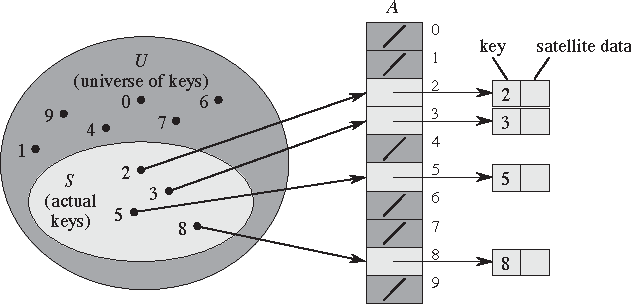
\includegraphics[width=0.6\linewidth]{direct_access_table.pdf}
    \caption{Direct access table}
    \label{fig:direct_access_table}
\end{figure}

\begin{figure}[htbp]
    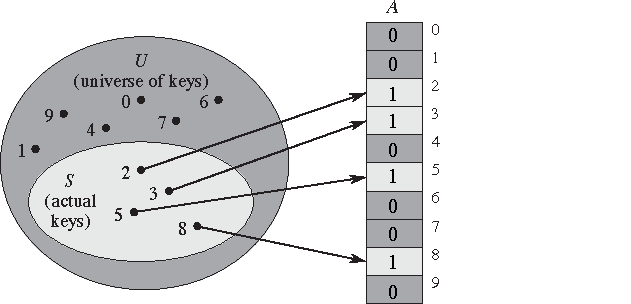
\includegraphics[width=0.6\linewidth]{bitvector_direct_access_table.pdf}
    \caption{Bit vector direct access table}
    \label{fig:bitvector_direct_access_table}
\end{figure}

\begin{codebox}
    \Procname{$\proc{Search}(A,k)$}
    \li $\Return$ $A[k]$
\end{codebox}

\begin{codebox}
    \Procname{$\proc{Insert}(A,x)$}
    \li $A[x.key] = x$
\end{codebox}

\begin{codebox}
    \Procname{$\proc{Delete}(A,x)$}
    \li $A[x.key] = \textsc{nil}$
\end{codebox}

Each of the three operations above takes constant time $O(1)$.

Alternatively, we can use value $1$ to indicate the presence of element at a given slot, and value $0$ to denote the absence of element at a given slot. The resulting data structure called a bit vector direct access table. \index{bit vector direct access table}

\chapter{Binary Search Trees}
\section{Binary Search Tree}

In this section, we will review some definition and properties of binary search trees.

\section{Searching in BST}

\section{Insertion}

\section{Deletion}

Deletion is the trickiest operation for BST.

\chapter{Balanced Search Trees}
\section{Balanced Trees}

There are two different ways of defining balancedness of a binary tree: weight balance and height balance. In this chapter, we will mainly focus on height balanced trees. As it turns out, weight balance is a more strict requirement than height balance, and weight balance implies height balance. Since the runtime complexity of binaryy tree operations are height-dependent, both definitions should give us $O(\lg n)$ time on most operations.

\begin{definition}[Height Balancedness] \index{height balanced}
    A binary tree is height balanced if for every node in the tree, the height of its left and right subtrees differ by at most one.
\end{definition}

\begin{definition}[Weight Balancedness] \index{weight balanced}
    A binary tree is weight balanced if for every node in the tree, the number of nodes of its left and right subtrees differ by at most one.
\end{definition}

\begin{corollary}
    Weight-balanced binary trees are height-balanced.
\end{corollary}

In this section we will look at a few height balanced search tree including red-black trees, AVL (Adelson-Velskii and Landis) trees, 2-3 trees, and B-trees which is a more general form of 2-3 trees. The first two are binary trees while 2-3 tree and B-tree are not necessarily binary.
\section{Red-Black Tree}

\subsection{Definition and Properties}

\vspace{\parskip}

\begin{definition}[Red-Black Tree] \index{red-black tree}
    A red-black tree is a binary search tree in which every node is either red or black and satisfies the following properties:
    \begin{enumerate}
        \item The root is black
        \item Every leaf node (\textsc{nil} node) is black
        \item If a node is red, then both its children are black
        \item For each node, all paths from the node to descendant leaves (\textsc{nil} nodes) contain the same number of black nodes
    \end{enumerate}
    Alternatively, the properties can be stated without using the \textsc{nil} node.
    \begin{enumerate}
        \item The root is black
        \item A red node has no red children
        \item Every path from the root to a node with at most one child contains the same number of black nodes
    \end{enumerate}
\end{definition}

Figure \ref{fig:rbtree} illustrates the properties of red-black trees.

\begin{figure}[hp]
    \centering
    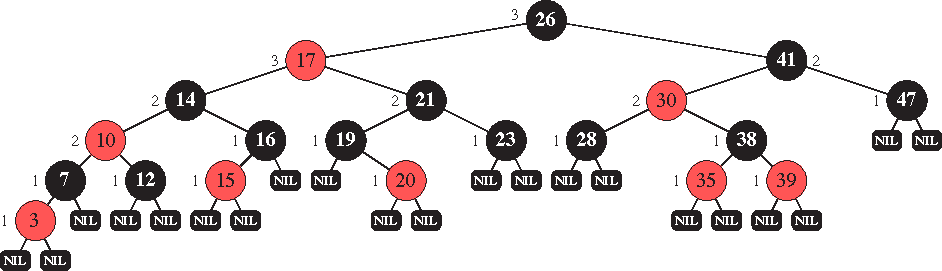
\includegraphics[width=\linewidth]{rbtree_nil.pdf}
    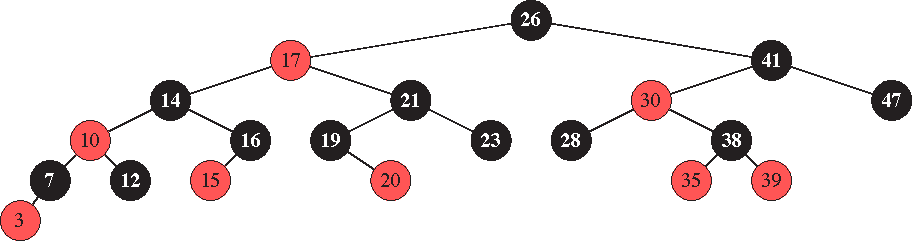
\includegraphics[width=\linewidth]{rbtree.pdf}
    \caption{Red-black trees. The first tree is represented with the \textsc{nil} sentinel node. The second tree is without the \textsc{nil} node. The two trees are equivalent and both satisfies the red-black tree properties.}
    \label{fig:rbtree}
\end{figure}

\begin{lemma}
    The number of nodes in a red-black tree of height $h$ is at least $2^{\left\lceil (h+1)/2 \right\rceil} - 1$.
\end{lemma}

\begin{proof}

    A red-black tree of height $h$ has a path of length $h$ from the root to a leaf node. This path contains $h+1$ nodes, the first of which is black. Since it does not contain two consecutive red nodes, the path contains at least $b = \left\lceil (h+1)/2 \right\rceil $ black nodes (i.e. at least half of the nodes on that path are black). Hence, every path from the root to a node with at most one child contains at least $b$ black nodes.
    It suffices to prove that there are at least $2^b-1$ black nodes in a red-black tree of height $h$ such that the number of black nodes in the path from the root to a leaf node is $b$. 

    \textsc{Base Case:} If the height of the tree is $0$, then the number of nodes is $1$.

    \textsc{Inductive Step:} Let $h \in \N$ be arbitrary. Assume that for all tree with height $h' < h$, there are $2^{b'}-1$ black nodes where $b'$ is the number of black nodes in the path from the root of that tree to a leaf node. 

    Consider an arbitrary tree $T$  with height $h$ with two subtrees. It follows that there are $b = \left\lceil (h+1)/2 \right\rceil$ black nodes from the root of the tree to a leaf node. If the subtree has a black root, then the path going from the root of the subtree to a leaf contains $b-1$ black nodes. If the root is red, then the path contains $b$ black nodes. Therefore, the number of black nodes in the path from the root of the tree to a leaf node is $b-1$ or $b$. Then, by induction hypothesis, the number black nodes in each subtree is at least $2^{b-1}-1$.

    Since the root of a red-black tree is black, the number of black nodes in $T$ is the number of nodes in the left subtree plus the number of nodes in the right subtree plus the root node.

    $$
    \left( 2^{b-1}-1 \right) + \left( 2^{b-1}-1 \right) + 1 = 2^{b}-1
    $$

    By induction, the number of black nodes in a red-black tree of height $h$ is at least $2^{b}-1 = 2^{\left\lceil (h+1)/2 \right\rceil} - 1$.

\end{proof}

\begin{corollary}
    A red-black tree with $n$ nodes has height $h \leq 2\log_2 (n+1)-1$. 
\end{corollary}

It follows immediately from this corollary that the $\textsc{Search}$ operation will run in $O(\lg n)$ time on a red-black tree.

\subsection{Rotations}

It is obvious that $\textsc{Insert}$ and $\textsc{Delete}$ will also run in $O(\lg n)$ time, but the resulting tree may not satisfy the red-black tree properties, meaning that the tree after insertion and deletion of nodes may not be a red-black tree. We can fix this using a technique known as rotation.

\subsubsection{Case 1}

\begin{figure}[htbp]
    \centering
    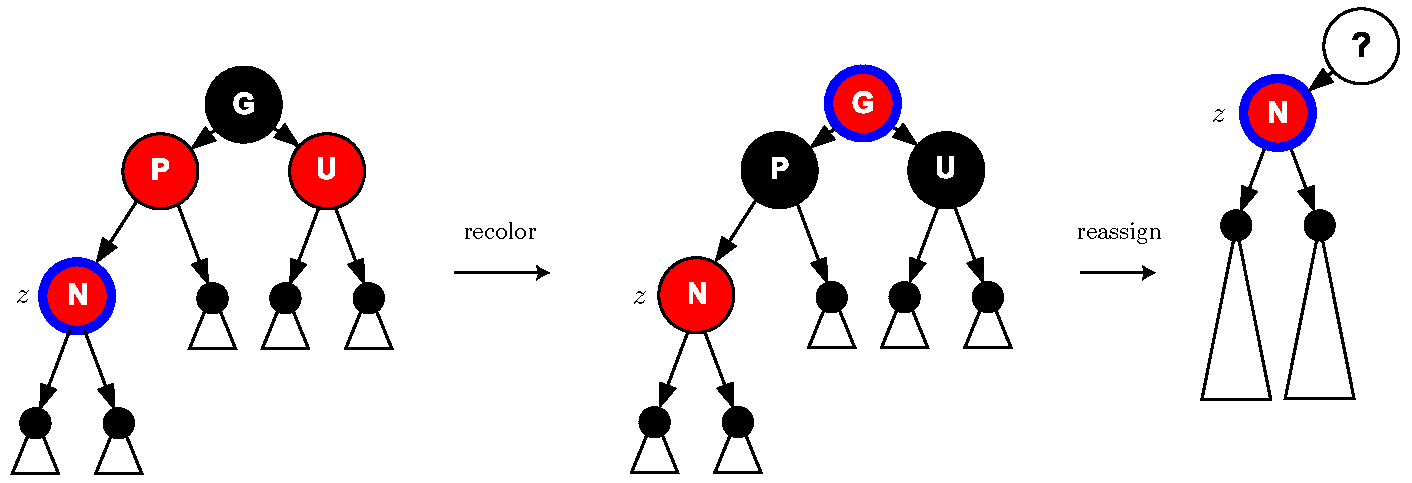
\includegraphics[width=0.9\linewidth]{rbtree_case1.pdf}
    \caption{<caption>}
    \label{fig:rbtree_case1}
\end{figure}

\subsubsection{Case 2}

\begin{figure}[htbp]
    \centering
    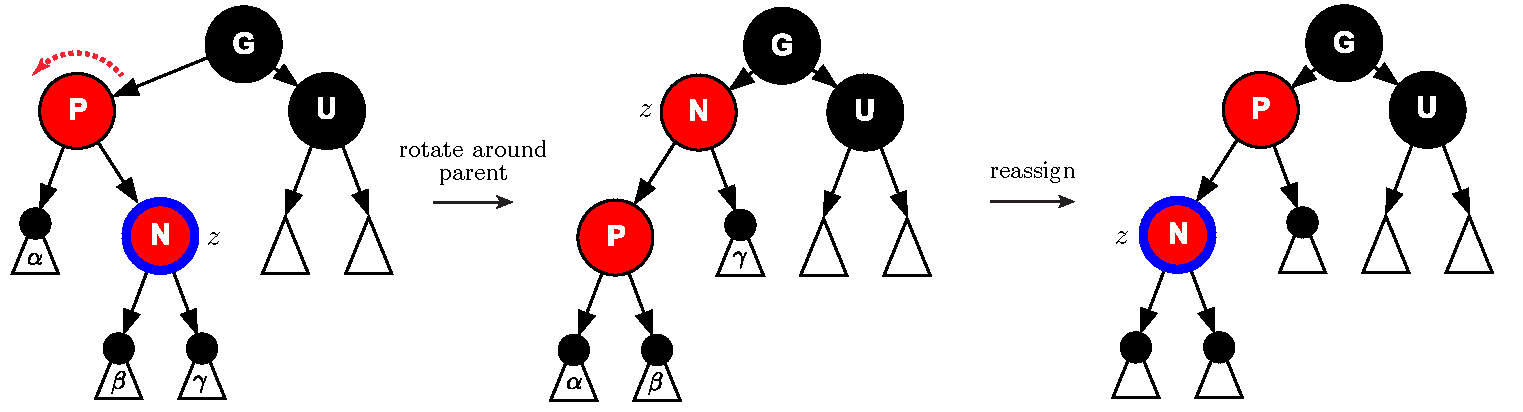
\includegraphics[width=0.9\linewidth]{rbtree_case2.pdf}
    \caption{<caption>}
    \label{fig:rbtree_case2}
\end{figure}

\subsubsection{Case 3}

\begin{figure}[htbp]
    \centering
    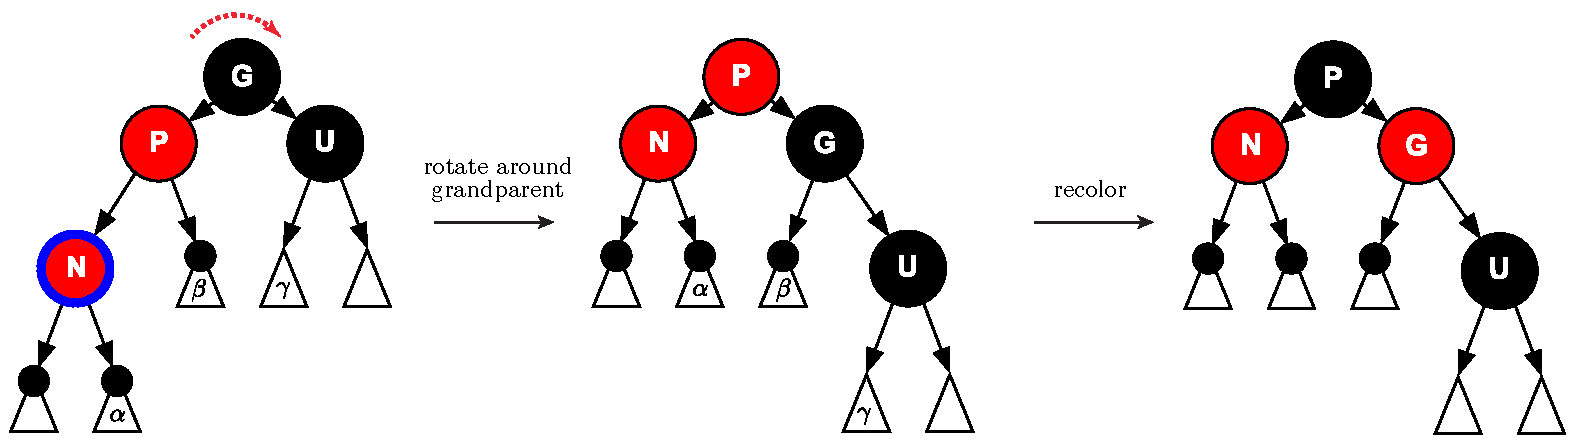
\includegraphics[width=0.9\linewidth]{rbtree_case3.pdf}
    \caption{<caption>}
    \label{fig:rbtree_case3}
\end{figure}
\section{AVL Tree}

\section{B-Tree}

\subsection{2-3 Tree}

\vspace{\parskip}

\begin{definition} \index{2-3 tree}
    A search tree is a \textbf{2-3 tree} if every internal node has either two children with one element, or three children with two elements. Leaf nodes of a 2-3 tree have no children and one or two elements. More formally, a tree $T$  is a 2-3 tree if and only if one of the following is true:
    \begin{itemize}
        \item $T$ is empty
        \item $T$ has one element $a$ and two children $p,q$ ($p$ being the left child and $q$ being the right child). $p$ and $q$ are 2-3 trees of the same height, and $a$ is greater than every element in $p$, and $a$ is less than every element in $q$ 
        \item $T$ has two elements $a < b$ and three children $p,q,r$ (left, middle, right children, respectively). $p$ and $q$ are 2-3 trees of the same height; and $a$ is greater than every element in $p$ and less than every element in $q$; and $b$ is greater than every element in $q$ and less than every element in $r$.
    \end{itemize}
    \begin{center}
        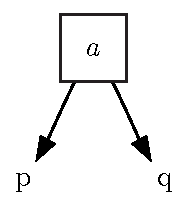
\includegraphics[width=0.15\linewidth]{2-3tree_2node.pdf} 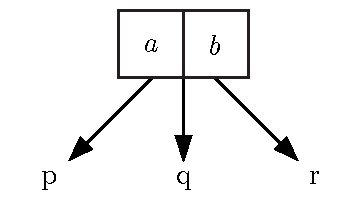
\includegraphics[width=0.3\linewidth]{2-3tree_3node.pdf}
    \end{center}
\end{definition}

\chapter{Augmenting Data Structures}
\section{Augmenting Data Structures}

For many problems, it is not enough to use only the elementary data structures such as linked list, hash table, or binary tree. But for most of those problems, we don't need to reinvent the wheel. Instead, we can augment the data structures we already have along with some additional information.

\section{Order Statistics With Red-Black Trees}

\section{Steps To Create Augmented Data Structures}

To create augmented data strucutres, we typically follow these four steps:

\begin{enumerate}
    \item choose an underlying data structure
    \item determine additional information to be maintained
    \item verify that the additional information can be maintained by update operations (or basic steps of update operations, e.g. rotations)
    \item develop new operations
\end{enumerate}

\begin{theorem}[Augmenting Red-Black Tree]
    Let $f$ be a field augmenting each node of a red-black tree and suppose that $x.f$ can be computed using information in node $x$, $x.left$, and $x.right$, possibly including $x.left.f$ and $x.right.f$. Then, the $f$ field can be maintained in all nodes during insertion and deletion without asymptotically affecting the $O(\lg n)$ performance of these operations.  
\end{theorem}

\textit{Proof Idea.} A change to $x.f$ only propagates to $y.f$ for the ancestors $y$ of $x$. Since the height of a red-black tree is $O(\lg n)$, at most $O(\lg n)$ nodes have their $f$ fields changed an each change takes $O(1)$ time.

\chapter{Priority Queue and Heap}
\section{Priority Queue} \index{priority queue}

\subsection{Priority Queue ADT}

The priority queue ADT is a data type that stores a collection of items with priorities (keys) that supports the following opeations:

\begin{itemize}
    \item \textsc{Insert}($Q, x$) inserts the element $x$ into the priority queue $Q$.
    \item \textsc{Maximum}($Q$) returns the element of $Q$ with the largest key.
    \item \textsc{Extract-Max}($Q$) removes and returns the element of $q$ with the largest key.
    \item \textsc{Increase-Key}($S,x,k$) increases the value of element $x$'s key into the new value $k$, assuming that $k \geq x$.
\end{itemize}

Priority queue allows us to access the element with largest (if max-priority queue) or smallest (if min-priority queue) more efficiently. It has many applications in computer science, such as: job scheduling in operation systems, bandwith management, or finding minimum spanning tree of a graph, etc.

\subsection{Primitive Implementation Using Linked Lists}

We can have a naive implementation of a priority queue simply using a sorted linked list, which has the following time complexity:
\begin{itemize}
    \item \textsc{Insert}($Q, x$): $\Theta(n)$ in the worst case. We have to linearly search the correct location of insertion.
    \item \textsc{Maximum}($Q$): $\Theta(1)$ by returning the head of the list.
    \item \textsc{Extract-Max}($Q$): $\Theta(1)$ by removing and returning the head of the list.
    \item \textsc{Increase-Key}($S,x,k$): $\Theta(n)$ in the worst case. Need to move element to new location after increase.
\end{itemize}

However, we want to have something that is more efficient than $\Theta(n)$. As it turns out, by putting the elements in a specific way, we can achieve worst-case time complexity of $\Theta(\log n)$ for \textsc{Insert}, \textsc{Extract-Max}, and \textsc{Increase-Key}. Even better, we can show that the amortized complexity of \textsc{Insert} is $\Theta(1)$ and \textsc{Extract-Max} is $\Theta(\log n)$.

\section{Heap} \index{heap}

\subsection{Types of Binary Trees}

Before starting to formally define heaps, let's review some definitions about binary trees. 

\begin{definition}[Full Binary Tree] \index{full binary tree}
    A full binary tree (sometimes proper binary tree or 2-tree) is a tree in which every node other than the leaves has two children. 
\end{definition}

\begin{definition}[Heap-Shape] \index{complete binary tree} \index{heap shape}
    A binary tree is in heap-shape if every level of the binary tree, except possibly the last, is completely filled, and all nodes are as far left as possible.

    Importantly, a binary tree in heap-shape with $n$ nodes has $\left\lfloor n / 2 \right\rfloor$ internal nodes (nodes that are not leaves).
\end{definition}

\begin{definition}[Complete Binary Tree] \index{perfect binary tree}
    A perfect binary tree is a binary tree in which all interior nodes have two children and all leaves have the same depth or same level.
\end{definition}

A note on the terminologies: some instructors and textbooks refer to a binary tree in heap-shape as ``complete binary tree'', and call a complete binary tree ``perfect binary tree''. In these notes, we will use ``heap shape'' and ``complete binary tree''. Unfortunately, both sets of terminologies are accepted and widely used.

\begin{figure}[h!]
    \centering
    \tikzset{every tree node/.style={minimum width=1em,draw,circle},
         blank/.style={draw=none},
         edge from parent/.style=
         {draw,edge from parent path={(\tikzparentnode) -- (\tikzchildnode)}},
         level distance=2em}
    \vcenteredhbox{
        \begin{tikzpicture}
            \Tree [.{} [.{} {} [.{} {} {} ] ]
            {} ]
        \end{tikzpicture}
    }
    \hfil
    \vcenteredhbox{
        \begin{tikzpicture}
            \Tree [.{} [.{} {} {} ]
            [.{} {} {} ] ]
        \end{tikzpicture}
    }
    \hfil
    \vcenteredhbox{
        \begin{tikzpicture}
            \Tree [.{} [.{} {} {} ]
            [.{} {} \edge[blank]; \node[blank]{}; ] ]
        \end{tikzpicture}
    }
    \caption{From left to right: full binary tree, binary tree in heap shape, complete binary tree.}
\end{figure}

Conveniently, a binary tree in heap-shape can be represented as an array.

\begin{figure}[htbp]
    \centering
    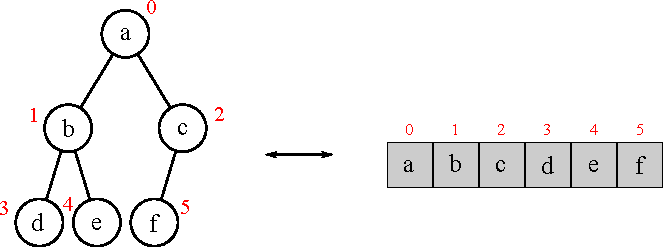
\includegraphics[width=0.6\linewidth]{figures/heap_as_arr.pdf}
    \caption{A heap-shaped binary tree and its corresponding array representation}
\end{figure}

Assuming that we index from 0, we can compute the indices of each node's parent, left, and right child.

\textsc{Parent}(i) = $\left\lfloor (i-1) / 2 \right\rfloor$ \\
\textsc{Left}(i) = $(2i)+1$ \\
\textsc{Right}(i) = $(2i)+2$

If we index from 1, the indices are calculated as follows:

\textsc{Parent}(i) = $\left\lfloor i / 2 \right\rfloor$ \\
\textsc{Left}(i) = $2i$ \\
\textsc{Right}(i) = $2i+1$

\subsection{Heap Property}

Then, we can define a max-heap as a binary tree in heap-shape with the max-heap property.

\begin{definition}[Max-heap Property] \index{max-heap property} \index{max-heap}
    In a max-heap represented by the array $A$ , the max-heap property is that for every node $i$ other than the root,
    \[
        A[\textsc{Parent}(i)] \geq A[i]
    .\]
    that is, the value of a node is at most the value of its parent.
\end{definition}

The max-heap property guarantees that the largest element in a heap is always stored at its root.

For our heap implementation, we will include the following operations: \proc{Insert}, \proc{Maximum}, \proc{Extract-Max}, \proc{Increase-Key}, \proc{Max-Heapify}, \proc{Build-Max-Heap}. The first few operations allow us to use heap to implement the priority queue ADT, and in addition to those, \proc{Build-Max-Heap} allows us to produce a max-heap from an unordered array.

\section{Maintaining the Heap Property}

Given an array $A$ and index $i$, \proc{Max-Heapify} will correct a single violation of the max-heap property in the subtree with $i$ as its root. To implement \proc{Max-Heapify}, we use a technique called ``trickle down''.

First, assume that the trees rooted at $\proc{Left}(i)$ and $\proc{Right}(i)$ are max-heaps. If element $A[i]$ violates the max-heap property, we correct thie violation by ``trickling'' element $A[i]$ down the tree until it reaches the correct position. By doing so, we can make the subtree rooted at index $i$ a max-heap. In every trickle-down step, swap $A[i]$ with its largest child.

\begin{codebox}
    \Procname{$\proc{Max-Heapify}(A,i)$}
    \li $l = \proc{Left}(i)$
    \li $r = \proc{Right}(i)$ 
    \li \If $l \leq A.heapsize$ and $A[l] > A[i]$
    \li \Then $largest = l$
    \li \Else $largest = i$
    \End
    \li \If $r \leq A.heapsize$ and $A[r] > A[largest]$ 
    \li \Then $largest = r$
    \End
    \li \If $largest \neq i$
    \li \Then exchange $A[i]$ with $A[largest]$
    \li       $\proc{Max-Heapify}(A,largest)$
    \End 
\end{codebox}

\subsection{Correctness of \proc{Max-Heapify}}

\subsection{Running Time of \proc{Max-Heapify}}

\section{Inserting Into Max-Heap}

To insert into a max-heap while maintaining the heap property, we use a similar technique. We first append the new element to the end of the heap. The new element will become the right-most leaf at the last level. Then, we check if the element is already at the right position. If not, we ``bubble'' the element up the tree, until it reaches the correct position.

\section{Build Heap From Unsorted Array}

\begin{codebox}
    \Procname{$\proc{Build-Max-Heap}(A)$}
    \li $A.heapsize = A.length$
    \li \For $i = \left\lfloor A.length / 2 \right\rfloor$ \textbf{downto} 1
    \li \Then $\proc{Max-Heapify}(A,i)$
    \End
\end{codebox}


The reason we start calling \proc{Max-Heapify} at $\left\lfloor A.length / 2 \right\rfloor$ is because elements beyond that $A[n / 2+1, \cdots, n]$ are all leaves of the tree. Recall that for a heap-shaped binary tree with $n$ nodes, there are only $\left\lfloor n / 2 \right\rfloor$ internal nodes.

\subsection{Running Time of \proc{Build-Max-Heap}}

Each call of \proc{Max-Heapify} takes $O(\log n)$ time, and \proc{Build-Max-Heap} calls \proc{Max-Heapify} $O(n)$ times. Thus, the running time of \proc{Build-Max-Heap} is $O(n \log n)$. However, this upper bound is not tight. We will prove a tighter upper bound of $O(n)$.

{
    \setlength\columnsep{4em}
    \begin{multicols}{2}
        
        Note that \proc{Max-Heapify} takes $O(1)$ time for nodes tthat are one level above the leaves, and in general, it takes $O(k)$ for nodes that are $k$ levels above the leaves.
        We have $n / 4$ nodes at level 1, $n / 8$ at level 2, etc. At the root level, which is $\log_2 n$ levels above the leaves, we have only 1 node.

        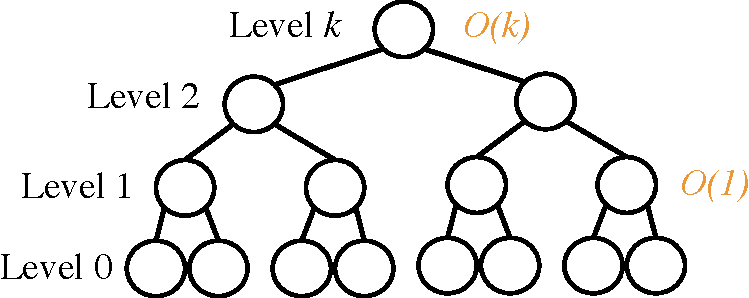
\includegraphics[width=\linewidth]{figures/build_max_heap.pdf}
    \end{multicols}
}

More generally, a heap with $n$ nodes has a height of $\left\lfloor \log_2 n \right\rfloor$ and at most $\left\lceil n / 2^{h+1} \right\rceil $ nodes at any height $h$. Hence, the total cost of \proc{Build-Max-Heap} can be written as
\[
\sum_{h=0}^{\left\lfloor \log_2 n \right\rfloor} \left\lceil \frac{n}{2^{h+1}} \right\rceil O(h) = O \left( n \sum_{h=0}^{\log_2 n} \frac{h}{2^h} \right)
.\]
The last summation is bounded by a constant, namely
\[
\sum_{h=0}^{\log_2 n} \frac{h}{2^h} \leq \sum_{h=0}^{\infty} \frac{h}{2^h} = 2 = O(1)
.\]
Thus,
\[
O \left( n \sum_{h=0}^{\log_2 n} \frac{h}{2^h} \right) = O(n) O(1) = O(n)
.\]

\section{Heapsort}

\begin{codebox}
    \Procname{$\proc{Heapsort}(A)$}
    \li \For $i = A.length$ \textbf{downto} 2
    \li \Then exchange $A[1]$ with $A[i]$
    \li $A.heapsize = A.heapsize - 1$
    \li $\proc{Max-Heapify}(A,1)$
    \End 
\end{codebox}

\chapter{Mergeable Heaps}


\part{Algorithm Analysis}

\chapter{Average Case Complexity and Randomized Algorithms}
\section{Basic Probability Theory}

\subsection{Sample Space and Events}

\vspace{\parskip}

\begin{definition}[Probability Space and Sample Space] \index{probability space} \index{sample space} \index{outcome} \index{event}
    A \textit{\textbf{probability space}} $(\Omega, \Prob)$ consists of a finite or countable set $\Omega$ called the sample space, and the probability function $\Prob:\; \Omega \to \R$ such that for all $\omega \in \Omega$, $\Prob(\omega) \geq 0$ and $\sum_{\omega \in \Omega} \Prob(\omega) = 1$. We cann an element $\omega \in \Omega$ a sample point, or \textit{\textbf{outcome}}, or \textit{\textbf{simple event}}.
\end{definition}

A sample space models some random experiment, where $\Omega$ contains all possible outcomes, and $\Prob(\omega)$ is the probability of the outcome $\omega$. We always talk about probabilities in relation to a sample space.

\begin{definition}[Event]
    An event $A$ is a set of outcomes, $A \subseteq \Omega$. We define the probability of an event $A$ to be the sum of the probabilities of its elements
    $$
    \Prob(A) = \sum_{\omega \in A} \Prob(\omega)
    $$ 
\end{definition}

If we have $\Prob(\omega) = \Prob(\omega')$ for all distinct $\omega, \omega' \in \Omega$, we say that the probability is uniform over $\Omega$.

\subsection{Properties of Probability Functions}

\vspace{\parskip}

\begin{definition}[Complement]
    The complement of an event $A$ is
    $$
    \overline{A} = \Omega \setminus A
    $$
    The complement of $A$ is also denoted by $\text{not }A$. 
\end{definition}

\begin{theorem}
    $$
    \begin{aligned}
        \Prob(\overline{A}) &= 1 - \Prob(A) \\
        \Prob(A \cup B) &= \Prob(A) + \Prob(B) - \Prob(A \cap B) \\
        \Prob(A \cup B) &\leq \Prob(A) + \Prob(B)
    \end{aligned}
    $$
    It can then be proved by induction that
    $$
    \Prob(A_1 \cup A_2 \cup \cdots \cup A_k) \leq \Prob(A_1) + \Prob(A_2) + \cdots + \Prob(A_k)
    $$
    for any events $A_1, \cdots A_k$.
\end{theorem}

We say that two events $A$ and $B$ are disjoint or mutually exclusive if $A \cap B = \emptyset$. If $A$ and $B$ are disjoint, $\Prob(A \cup B) = \Prob(A) + \Prob(B)$.

\section{Conditional Probability and Independence}

Conditional probability allows us to compute the probability of some event given that we already know that some other events have occurred.

\begin{definition}[Conditional Probability] \index{conditional probability}
    The probability of an event $A$ conditional on an event $B$ is
    $$
    \Prob(A \mid B) = \frac{\Prob(A \cap B)}{\Prob(B)}
    $$
    given that $\Prob(B) > 0$. 
\end{definition}

\section{Average Case Analysis}

Let $A$ be an algorithm, and let
\[
t(x) = \text{number of steps taken by $A$ on input $x$}
.\] 

We know that the worst case time complexity of $A$ is
$$
T(n) = \max \{ t(x) \mid \text{$x$ has size $n$ } \}
$$

We can define the average case time complexity of $A$ as

\begin{definition}
    The average case time complexity of $A$ is
    $$
    T'(n) = \Expected [ t(x) \mid \text{$x$ has size $n$} ]
    $$
    If all inputs of size $n$ are equally likely, then
    $$
    T'(n) = \frac{\sum \{ t(x) \mid size(x) = n \}}{| x \mid size(x) = n |}
    $$
\end{definition}

In general, the average case time complexity is less than or equal to the worst case time complexity, that is $T'(n) \leq T(n)$ for all $n$.

The average case time complexity is dependent on the probability distribution of the inputs, which in turn can depends on the application where the algorithm is to be used. However, this is usually unknown, in which case, uniform distribution usually makes the analysis easier. For some applications, an algorithm with good average case behavior but bad worst case behavior is sufficient.

We follow the following steps before we can analyze the average case time complexity of an algorithm:

\begin{itemize}
    \item define the sample space of the inputs
    \item define the probability distribution function
    \item define any necessary random variables
\end{itemize}

\section{Average Case Analysis of Linear Search}

Consider the following algorithm for linear search in an unsorted array.

\begin{codebox}
    \Procname{$\proc{Linear-Search}(L,k)$}
    \li $j = 1$
    \li \While $j \leq n$ \Do
    \li \If $L[k] == k$
    \li \Then \Return $j$ \End
    \li $j = j + 1$ \End
    \li \Return 0 
\end{codebox}

It is obvious that the worst case complexity is $O(n)$ because there will be at most $n$ comparisons with the searching key $k$. Following the procedure introduced above, we can perform an average case complexity analysis.

\begin{enumerate}
    \item \textbf{Define sample space}: This will be the set of possible inputs that we are considering in our analysis. We define our sample space to be all pairs $(L,k)$ where $L$ is an input of size $n$ and $k$ is a key. Some observations on our choice of sample space:
    \begin{itemize}
        \item If we fix $L = [l_1, \cdots, l_n]$, then the sample space for $k$ is $[l_1,\cdots,l_n, \textsc{nil}]$ where $\textsc{nil}$ is used to indicate a value that is not in $L$. Hence, for a $L$ of size $n$, the sample space for $k$ contains $n+1$ sample points.
        \item The number of comparisons performed by $\proc{Linear-Search}(L,k)$ is the same for $(L,k)$ and $(L',k')$ if $k$ occurs in $L$ at the same position as $k'$ in $L'$.
        \item If $k$ and $k'$ are not in $L$, then $\proc{Linear-Search}(L,k)$ will also perform the same number of comparisons.
        \item The relative order between elements of $L$ does not matter since $\proc{Linear-Search}$ only performs equality tests, so choosing $L=[1,\cdots,n]$ is just as good as $L=[n,\cdots,1]$.
    \end{itemize}
    Hence, we can formally define our sample space as
    $$
    S_n = \{ (L,i) \mid i \in \{ \textsc{nil}, 1, \cdots, n \} \}
    $$
    where $L = [1,\cdots,n]$.
    \item \textbf{Probability distribution}: We choose uniform distribution, which means that every point in the sample space has the same probability $\displaystyle \frac{1}{n+1}$.
    \item \textbf{Define random variable}: Let $t_n:\; S_n \to \N$ be such that $t_n(i)$ is the number of comparisons performed when the input is $(L,i)$ where
    $$
    t_n(i) = \begin{cases}
        i & \text{for $i=1,\cdots,n$ } \\
        n & \text{for $i=0$ }
    \end{cases}
    $$
    \item \textbf{Analysis}:

    For the uniform distribution,
    $$
    \begin{aligned}
        T'(n) &= \Expected[t_n] = \frac{\sum \{ t_n(L,i) \mid i = \textsc{nil},\cdots,n \}}{n+1} \\
        &= \frac{n + \sum_{i=1}^n i}{n+1} \\
        &= \frac{n + \frac{n(n+1)}{2}}{n+1} \\
        &= \frac{n}{2} + \frac{n}{n+1} \\
        &< \frac{n}{2} + 1 
    \end{aligned}
    $$
    Hence, $\displaystyle T'(n) \in O(\frac{n}{2})$.
\end{enumerate}

\section{Average Case Analysis of Quick Sort}

Quicksort is ued to sort a multi-set of elements $S$ from a totally ordered domain. The pseudocode for quicksort is shown below.

\begin{codebox}
    \Procname{$\proc{Quicksort}(S)$}
    \li \If $|S| \leq 1$
    \li \Then \Return $S$ \End
    \li $pivot = \text{select a pivot}$
    \zi \Comment partition $S$ into $L$, $E$, and $G$ such that $L$ contains all elements less than $pivot$
    \zi \Comment $E$ contains all elements equal to $pivot$, and $G$ contains all elements greater than $pivot$
    \li $L,E,G = \proc{Partition}(S,pivot)$
    \li \Return $\proc{Quicksort}(L) + E + \proc{Quicksort}(G)$
\end{codebox}

In practice, we often choose the first element of $S$ as the pivot. The worst case time complexity of quicksort is $O(n^2)$ because it has to partition the input $S$ into three parts, $L$, $E$, and $G$, which gives us this recurrence.
$$
T(n) = T(n-1) + T(0) + \Omega(n) \in O(n^2)
$$
Following the procedure introduced above, we can perform an average case complexity analysis. In \proc{Quicksort}, only the relative order of the elements matter, not their actual values.

\begin{enumerate}
    \item Define sample space: $S_n = \text{all permutations of $\{1,\cdots,n\}$}$
    \item Probability distribution: We know that $\left| S_n \right| = n!$. Assuming uniform distribution, we have
    $$
    \Prob[\pi] = \frac{1}{n!} \qquad \text{for all $\pi \in S_n$}
    $$
    \item Random variables: Let $t_n: \; S_n \to \N$ be the random variable such that
    $$
    t_n(i) = \text{number of element comparison performed by $\proc{Quicksort}(S)$}
    $$
    \item Analysis: Let $T'(n) = \Expected[t_n]$. Let $X_{ij} \; S_n \to \{0,1\}$ be an indicator random variable such that $X_{ij}(\pi) = 1$ if and only if elements $i$ and $j$ are compared during $\proc{Quicksort}(\pi)$. Since no pair of elements is compared more than once,
    $$
    t_n(\pi) = \sum_{1 \leq i < j \leq n} X_{ij}(\pi),
    $$
    and
    $$
    \begin{aligned}
        T'(n) = \Expected[t_n] &= \sum_{1 \leq i < j \leq n} \Expected[X_{ij}] & {\text{by linearity of expectation }} \\
        &= \sum_{1 \leq i < j \leq n} \Prob[X_{ij} = 1] & {\text{since $X_{ij}$ is an indicator variable }}
    \end{aligned}
    $$
    In $\proc{Quicksort}(\pi)$, as long as no element in $\{i, \cdots, j\}$ is chosen as a pivot, these elements will stay together, either all going to $L$, or all going to $G$ in recursive calls. 

    Eventually, one of the elements in $\{i, \cdots, j\}$ is chosen as pivot. Suppose that $p$ is the first of the elements in $\{ i, \cdots, j \}$ that is chosen as pivot. If $i < p < j$, then $i$ and $j$ are not compared during $\proc{Quicksort}$. If $p=i$ or $j=j$, then $i$ and $j$ are compared.
    
    There are $j-i+1$ possibilities for $p$ to be chosen as pivot. Among those possible choices, $X_{ij} = 1$ for two possibilities, and $X_{ij} = 0$ for the rest. Since all permutations of the inputs are equally likely, each of these possibilities for $p$ is equally like and has probability of $\displaystyle \frac{1}{j-i+1}$.

    Hence,
    $$
    \Prob[X_{ij} = 1] = \frac{2}{j-i+1}
    $$

    Using this, we can rewrite $T'(n)$ as with $k = j-i+1$ 
    $$
    \begin{aligned}
        T'(n) &= \Expected[t_n] \\
        &= \sum_{1 \leq i < j \leq n} \Prob[X_{ij} = 1] \\
        &= \sum_{i=1}^n \sum_{j=i+1}^{n-1} \frac{2}{j-i+1} \\
        &= \sum_{i=1}^n \sum_{k=1}^{n-1} \frac{2}{k+1} & \text{substituting $k$} \\
        &< \sum_{i=1}^n \sum_{k=1}^n \frac{2}{k} \\
        &= \sum_{i=1}^n O(n\, \lg n) & \text{harmonic series} \\
        &= O(\lg n)
    \end{aligned}
    $$

    Therefore, the average case time complexity of quicksort is $O(n \, \lg n)$.
\end{enumerate}

From this analysis, we notice that the average case time complexity for quicksort is much smaller than the worst case time complexity. If the actual distribution of inputs is close to uniform distribution, then the average case time complexity will serve as a more realistic estimate of running time. But problem arises when the actual distribution is not uniform. To solve this issue, we can modify the quicksort algorithm to use a randomized pivot selection.

\section{Randomized Quicksort}

In randomized quicksort, we randomly pick the pivot instead of using the first element of $S$. Pick each element of $S$ to be the pivot with probability of $\displaystyle \frac{1}{|S|}$ using a random number generator. 

\begin{codebox}
    \Procname{$\proc{Randomized-Quicksort}(S)$}
    \li \If $|S| \leq 1$
    \li \Then \Return $S$ \End
    \li $r = \proc{Random}(1,|S|)$
    \li $pivot = S[r]$ 
    \zi \Comment partition $S$ into $L$, $E$, and $G$ such that $L$ contains all elements less than $pivot$
    \zi \Comment $E$ contains all elements equal to $pivot$, and $G$ contains all elements greater than $pivot$
    \li $L,E,G = \proc{Partition}(S,pivot)$
    \li \Return $\proc{Randomized-Quicksort}(L) + E + \proc{Randomized-Quicksort}(G)$
\end{codebox}

$\proc{Random}(i,j)$ will return a number in $\{i, i+1, \cdots, j-1, j\}$ each equally likely, assuming $i \leq j$.

Let $t(I,p)$ denote the running time of algorithm $A$ on input $I$ with the sequence of random choices $p$. Then, the expected running time of algorithm $A$ on input $I$ is
$$
\Expected_p \left[ t(T,p) \right] = \sum_e \Prob [p] t(I,p)
$$

The worst case expected time complexity of algorithm $A$ is
$$
T(n) = \max_{I \in S_n} \Expected_p \left[ t(I,p) \right]
$$
where $S_n$ is the set of all inputs of size $n$.

Note that the worst case complexity does not depend on any assumption about the input distribution.

\chapter{Hashing}
\section{Hashing and Hash Function} \index{hashing}

Let $U$ be the universe of possible keys, and let $m$ be the size of the hash table. Then, we say that
$$
h:\; U \to \{0, \cdots, m-1 \}
$$
is a hash function.

If two keys are mapped to the same location/bucket/slot by the hash function, we say that they collide.

Furthermore, if $|U| > m$, then by the pigeonhole principle, there are at least two keys that collide. And because in virtually all cases, $|U| > m$, collision is unavoidable. A well-chosen hash function will minimize the number of collisions, but we still need some means to resolve collisions.

\begin{remark}
    A fun fact about the etymology of the word ``hash'': it is said that the word ``hash'' originated from the french word ``hache'', which refers to the action of chopping something into pieces. Hashing, as we will see, involves the same notion of randomly chopping and mixing.
\end{remark}

\section{Resolving Collision}

Chaining put all elements in $S \subseteq U$ that hash to the same slot in a linked list.

We define the load factor $\alpha$ to be $\alpha = n/m$ where $n = |S|$ and $m$ is the number of buckets (slots) in the hash table. $\alpha$ is the average number of elements of $S$ stored in a slot of the hash table.

Let $n_i$ be the number of elements of $S$ in slot $i$. Then,
$$
\sum_{i=0}^{m-1} n_i = n
$$

In the worst case, hashing with chaining takes $\Theta(\max_{0 \leq i \leq m-1} n_i)$ in addition to the time to compute $h(x)$ (the hashing step).

From the analysis above, we know that $\max\{n_i\} = n$ if all elements of $S$ map to the same bucket.

If $|U| > m(n-1)$, then by the pigeonhole principle, there exists $S \subseteq U$ with $|S|=n$ such that all element of $S$ hash to the same bucket.

Overall, hashing with chaining without randomization has the following time complexity:
\begin{itemize}
    \item $\proc{Insert}(x)$: $O(1)$ assuming all linked lists are unsorted and $x \not\in S$
    \item $\proc{Delete}(p)$: $O(1)$ if list is doubly linked; if singly linked, then $O(n_i)$ where $n_i$ is the size of the bucket where $p$ is in.
\end{itemize}

\section{Universal Hashing}

We can achieve better time complexity by randomly choosing the hash function. There is a family of hash functions that we call the universal hash functions, which we will define as follows.

\begin{definition}[Universal Hashing] \index{universal hashing}
    Let $\mathcal{H}$ be a finite collection of hash functions that map a given universe $U$ into the range $\{0,\cdots,m-1\}$. Such a collection is said to be universal if for each pair of distinct keys, $k,l \in U$, the number of hash functions $h \in \mathcal{H}$ for which $h(k) = h(l)$ is at most $|\mathcal{H}|/m$. In other words, with a hash function randomly chosen from $\mathcal{H}$, the chance of a collision between distinct keys is not more than the chance $1/m$ of a collision if $h(k)$ and $h(l)$ were randomly and independently chosen from the set $\{0,\cdots,m-1\}$.

    That is, a finite set $\mathcal{H}$ of hash functions from $U \to [0,\cdots,m-1]$ is universal if for all $x \neq y \in U$
    $$
    \Pr_{h \in \mathcal{H}} [h(x) = h(y)] \leq \frac{1}{m}
    $$
    or equivalently,
    $$
    \left| \{ h \in \mathcal{H} \mid h(x) = h(y) \} \right| \leq \frac{|\mathcal{H}|}{m}
    $$
\end{definition}

Here are some examples of universal hashing families.

\begin{enumerate}
    \item $\mathcal{H}$ is the set of all functions from $U \to [0,\cdots,m-1]$ assuming $U$ is finite. Let $u = |U|$. Then, $|\mathcal{H}|=m^u$. For any distinct $x,y\in U$
    $$
    \left| \{ h \in \mathcal{H} \mid h(x) = h(y) \} \right| = m^{u-1} = \frac{|\mathcal{H}|}{m}
    $$
    since there are $m$ choices for which bucket each element of $U - \{y\}$ gets mapped to. So,
    $$
    \Pr_{h \in \mathcal{H}} [h(x) = h(y)] = \frac{1}{m}
    $$
    Therefore, $\mathcal{H}$ is universal.

    \item Let $p$ be prime and $U = \{0,\cdots,p-1\} = \Z_p$. And let
    $$
    h_{a,b}(x) = [(ax+b) \bmod p] \bmod m
    $$
    and
    $$
    \mathcal{H}_{p,m} = \{h_{a,b}:\, U \to [0,\cdots,m-1] \mid a,b \in U, a \neq 0 \}
    $$
    So $|\mathcal{H}_{p,m}| = p(p-1)$. We can prove that $\mathcal{H}_{p,m}$ is universal.

    \item Let $U = \{0, \cdots, 2^k-1\}$ and let
    $$
    h_a(x) = \left\lfloor \frac{ax \bmod 2^k}{2^{k-m'}} \right\rfloor
    $$
    This selects the $(k-m'+1)$th through $k$th least significant bits. In other words, we throw away everything in $ax$ except the $k$ least significant bits, and then remove $k-m$ least significant bits. The size of the hash table is $m=2^{m'}$.
    
    Let
    $$
    \mathcal{H}' = \{ h_a \mid 0 < a < 2^k,\, \text{$a$ is odd}\}
    $$
    We have $|\mathcal{H}'| = u/2$. $\mathcal{H}'$ is universal. The proof is more complicated.
\end{enumerate}

For each of the universal hash families, let's also take a look at their sizes
\begin{enumerate}
    \item $|\mathcal{H}| = m^u$. To specify a hash function in $\mathcal{H}$, we need $u\log_2 m$ bits. This is too big.
    \item $|\mathcal{H}_{p,m}| < u^2$. To specify a hash function $\mathcal{H}_{p,m}$, we need less than $2 \log_2 u$ bits.
    \item $|\mathcal{H}'| = u / 2$. To specify a hash function in $\mathcal{H'}$, wee need $(\log_2 u) - 1$ bits.
\end{enumerate}

\section{Analysis of Hashing with Chaining}

Fix $S \subseteq U$ where $|S|=n$. Pick $h \in \mathcal{H}$ randomly where $\mathcal{H}$ is a universal family of hash functions from $U \to \{0,\cdots,m-1\}$.

Let $x \in U$. Let $C_x:\, \mathcal{H} \to \N$ be such that
$$
C_x(h) = \text{the number of keys in $S$ that hash to $h(x)$}
$$
$C_x$ is a random variable that depends on the choice of $h$.

For each $y \in S$, let $C_{x,y}:\; \mathcal{H} \to \{0,1\}$ be the indicator random variable that is $1$ if and only if $h(x)=h(y)$.
$$
C_x(h) = \sum_{y \in S} C_{x,y}(h)
$$

\begin{theorem}[Expected Number of Collisions For Each Key in Universal Hashing]
    $$
    \Expected_{h\in\mathcal{H}}[C_x] \leq 1+\frac{n}{m} = 1 + \alpha
    $$
\end{theorem}

\begin{proof}
    If $y=x$, then $C_{x,y}(h)=1$ for all $h \in \mathcal{H}$ so $\Expected_{h\in\mathcal{H}}[C_x] = 1$.

    If $y \neq x$, then
    $$
    \begin{aligned}
        \Expected_{h\in\mathcal{H}}[C_{x,y}] &= \Pr_{h\in\mathcal{H}}[C_{x,y}(h) = 1] & \text{since $C_{x,y}$ is indicator variable} \\
        &= \Pr_{h\in\mathcal{H}}[h(x)=h(y)] \leq 1/m & \text{since $\mathcal{H}$ is universal}
    \end{aligned}
    $$
    Hence,
    $$
    \begin{aligned}
        \Expected_{h\in\mathcal{H}}[C_x] &= \sum_{y\in S}\Expected_{h\in\mathcal{H}}[C_{x,y}] & \text{by linearity of expectation} \\
        &\leq 1 + \sum_{y \in S-\{x\}} \frac{1}{m} \leq 1 + \frac{n}{m} = 1+\alpha
    \end{aligned}
    $$
\end{proof}

\begin{corollary}
    The worst-case expected search time for $x$ is $O(1+\alpha)$.
\end{corollary}

\begin{corollary}
    Starting with an initially empty hash table of size $m$, the worst-case expected time to handle any sequence of $s$ \proc{Insert}, \proc{Delete}, \proc{Search} operations containing $n = O(m)$ \proc{Insert} operations is $O(s)$. Hence, we can perform each operation in $O(1)$ time.
\end{corollary}

\section{Perfect Hashing} \index{perfect hashing}

$h$ is perfect for $S$ if for each element of $S$ hashes to a different slot (i.e. no collisions). For example,
$$
h(x) = x \bmod 5
$$
is perfect for $\{1,14,20\}$, but not for $\{1,9,14\}$.

For a static dictionary (where $S$ does not change with no \proc{Insert} and \proc{Delete}),then it may be worthwhile to find a perfect hash function for $S$. For example, it is useful to construct a perfect hash function if we are designing a compiler for a programming language, and our $S$ is the set of reserved keywords in the language.

\subsection{Constructing a Perfect Hash Functions}

Let $S$ be a set of $n$ keys. Let $\mathcal{H}$ be a universal family of hash functions. Let $C:\, \mathcal{H}\to\N$ be the random variable so that
$$
C(h) = \text{the number of collisions when $h$ is used to hash $S$}
$$
More formally,
$$
C(h) = \left| C_{x,y} \in S \mid x \neq y,\, h(x)=h(y) \right|
$$
where $C_{x,y}$ is defined similarly as the indicator variable that is $1$ if and only if $h(x)=h(y)$. 

\begin{lemma}[Expected Number of Collisions in Universal Hashing]
    $$
    \Expected[C] \leq \frac{{n \choose 2}}{m}
    $$
\end{lemma}

\begin{proof}
    $$C(h) = \sum \{ C_{x,y}(h) \mid x<y,\, x,y \in S \}$$
    By linearity of expectation,
    $$
    \begin{aligned}
        \Expected_{h \in \mathcal{H}} [C] &= \sum \{ \Expected_{h \in \mathcal{H} } [C_{x,y}] \mid x,y \in S,\, x < y\} \\
        &= \sum \{ \Pr_{h \in \mathcal{H}} [h(x)=h(y)] \mid x,y\in S,\, x<y\} \\
        &\leq \sum \{1/m \mid x,y \in S,\, x<y \} & \text{since $\mathcal{H}$ is universal} \\
        &= \frac{{n \choose 2}}{m} & \text{since there are ${n \choose 2}$ pairs of keys that may collide}
    \end{aligned}
    $$
\end{proof}

If $m > {n \choose 2}$, then $\Expected_{h \in \mathcal{H}}[C] < 1$. Since $C(h) \in \N$ for all $h \in \mathcal{H}$, this implies that there exists some $h \in \mathcal{H}$ such that $C(h) = 0$. This tells if we are willing to use $\Theta(n^2)$ space for the hash table, there exists a hash function $h \in \mathcal{H}$ that is perfect for $S$, so that \proc{Search} only takes only one step.

\begin{theorem}
    If $m > 2 {n \choose 2} = n(n-1)$, then
    $$
    \Expected_{h \in \mathcal{H}}[C] < \frac{1}{2}
    $$
    This means more than half of the functions in $\mathcal{H}$ is perfect for $S$.
\end{theorem}

The randomized algorithm for constructing a perfect hash function, we

\begin{codebox}
    \Procname{$\proc{Construct-Perfect-Hash}(\mathcal{H}, S)$}
    \li Pick $h \in \mathcal{H}$ uniformly at random.
    \li \For $s$ in $S$ \Do
        \li \If there is a collision \Then
        \li start over and try again
    \End \End
    \li \If no collision \Then
        \li \Return $h$ 
\end{codebox}

If $m > 2 {n \choose 2}$, the expected number of tries is less than 2, and the algorithm takes $O(2n)$ time to find a perfect hash function for $S$.

\subsection{FKS Hashing} \index{FKS hashing}

However, sometimes when the size of $S$ is large, the $O(n^2)$ space that our current perfect hashing table is not longer ideal. In this case, we want to use $m \in O(n)$ space for the hash table. Then,
$$
\Expected[C] = \frac{{n \choose 2}}{m} \in O(n)
$$
Some buckets will have size $>1$, but all buckets are likely to have size $O(\sqrt{n})$. Essentially, if a bucket have size $b$, there are at least $\displaystyle {b \choose 2}$ collisions. 

The idea is to use a perfect hash function to represent each bucket. If the size of bucket $i$ is $b$, we will use $b^2$ space for it. The resulting data structure is a 2-level hash. For $i=0,\cdots,m-1$, let $n_i(h) = \{ x \in S \mid h(x_i) = i \}$ be the number of keys in $S$ that get mapped to bucket $i$ by $h$. An example of the resulting hash table is shown in Figure \ref{fig:fks-hashing}.

$$
\sum_{i=0}^{m-1} n_i(h) = n
$$

\begin{figure}[htbp]
    \centering
    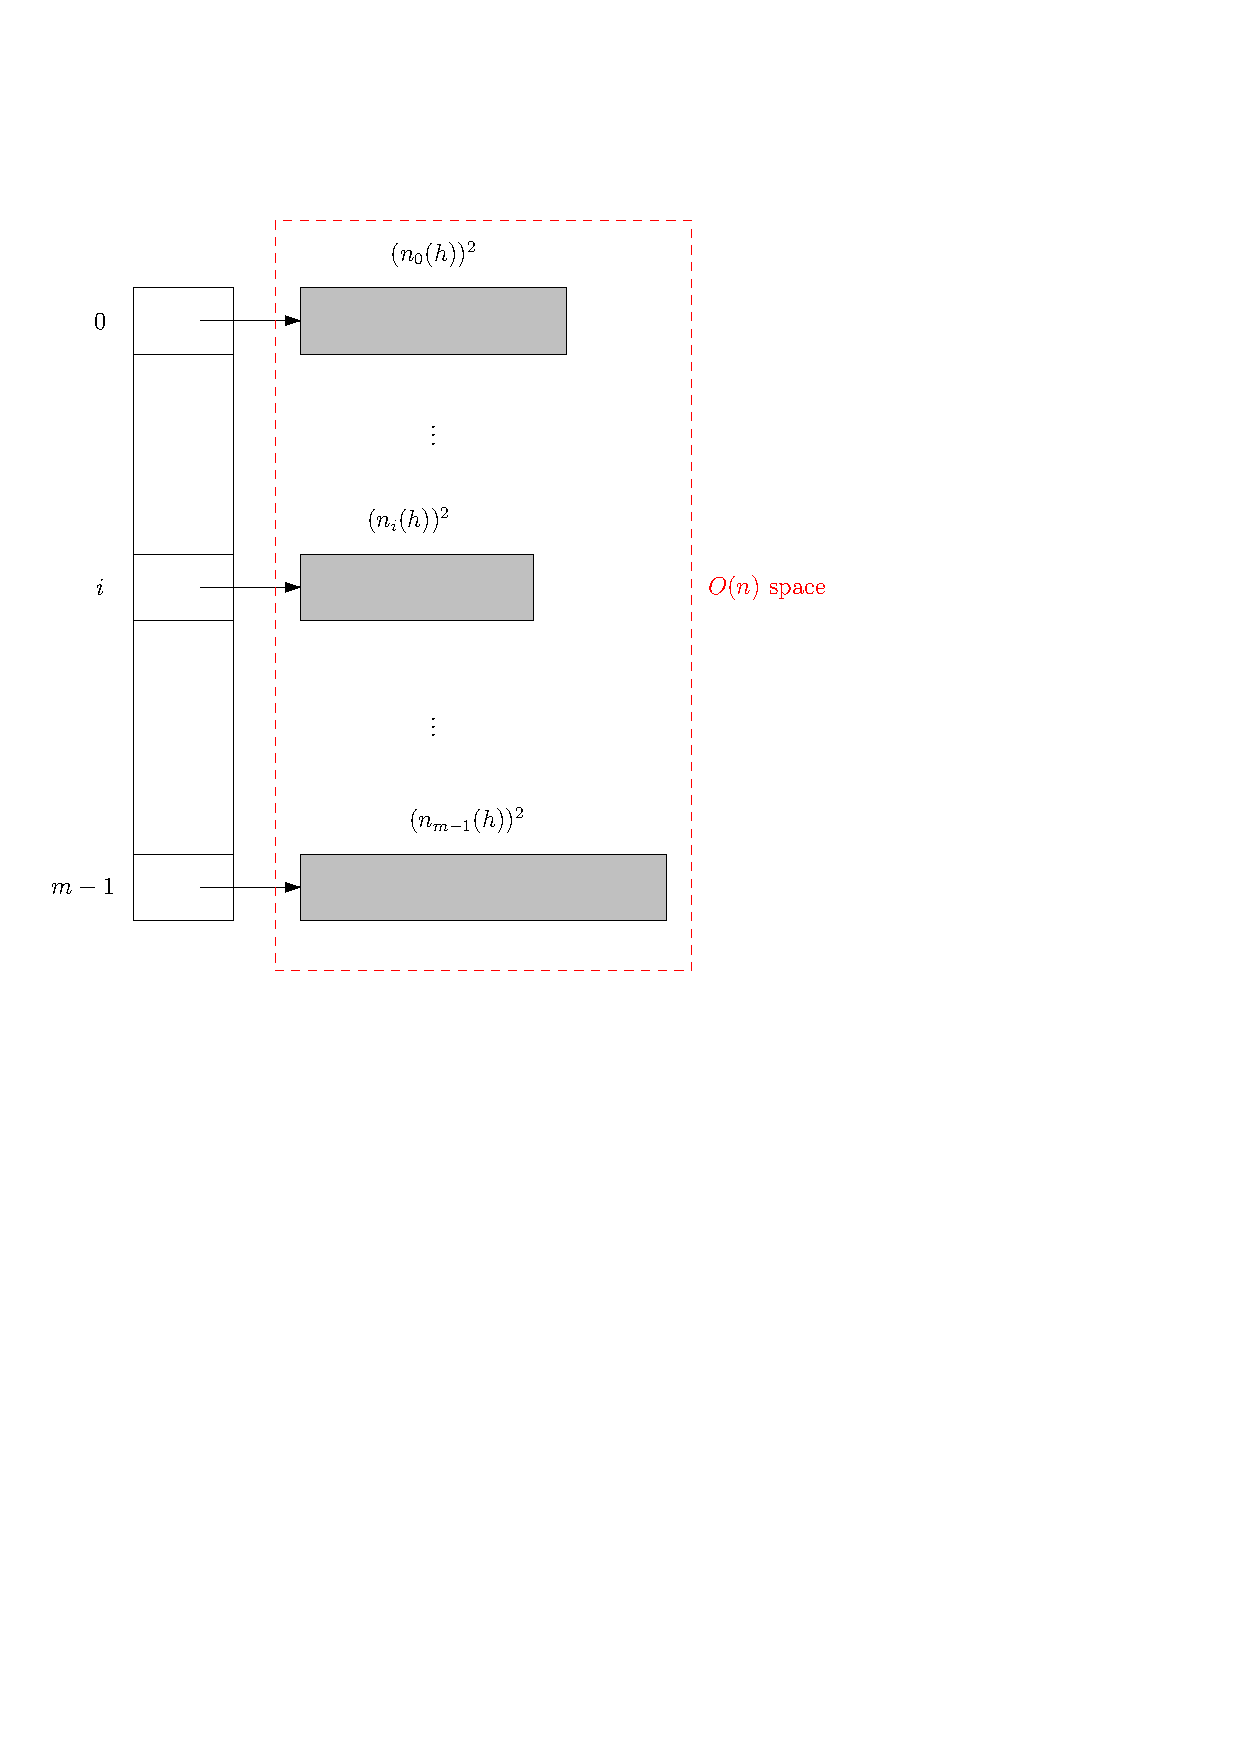
\includegraphics[width=0.5\linewidth]{fks-hashing.pdf}
    \vspace{2em}
    \caption{FKS 2-level hash table. As shown in the diagram and explained above, the length of each secondary hash table is $(n_i(h))^2$. }
    \label{fig:fks-hashing}
\end{figure}

The expected amount of space used by all the secondary hash tables can be computed as follows:

$$
\begin{aligned}
    C(h) &= \sum_{i=0}^{m-1} {n_i(h) \choose 2} \\
    &= \sum_{i=0}^{m-1} \frac{n_i(h)^2}{2} - \sum_{i=0}^{m-1} \frac{n_i(h)}{2} \\
    &= \frac{1}{2} \sum_{i=0}^{m-1} n_i(h)^2 - \frac{n}{2}
\end{aligned}
$$
By linearity of expectation,
$$
\begin{aligned}
    \Expected\left[ \sum_{i=0}^{m-1} n_i(h)^2 \right] &= 2 \Expected[C] + n \\
    &= 2\frac{{n \choose 2}}{m} + n \in \Theta(n) & \text{if $m \in \Theta(n)$ }
\end{aligned}
$$

$h$ itself is not a perfect hash function. For each non-empty bucket, find a hash function $h_i:\; U \to \{0,\cdots,m_i-1\}$, where $m_i = (n_i(h))^2$, that is perfect for the seconday hash table at bucket $i$ (i.e. perfect for the set $\{ x \in S \mid h(x) = i \}$).

\subsection{Representing FKS Hash Table}

In practice, we can represent the two-level FKS hash table for $S \subseteq U$ as a single array. Suppose that $U = \{ 0, \cdots, p-1 \}$. We use $\mathcal{H}_{p,m}$ for different values of $m$.

The first 3 locations of the array contain $m$, $a$, and $b$ used to specify the first-level hash function $h$. In particular, $m$ is the size of the first-level hash table; $a$ and $b$ are the parameters for the first-level table.

The next $m$ locations contain pointers to array corresponding to each second-level hash table.

Each second-level table is stored preceeded by the specifications of its hash function: $m_i = n_{i}(h_{a,b})$ and the parameter $a_i + b_i$ that specifies the perfect hash function $h_{a_i,b_i}$ for the $i$th secondary hahs table.

\begin{example}
    Let $p=31$. $U= \{0,\cdots,30\}$, $n=6$, and $S= \{2,4,5,15,18,30\}$, so $n=6$. Let the size of the first-level hash table be $m$.

    We randomly choose a hash function from $\mathcal{H}_{31,6}$ for the first-level table. Suppose that we end up getting
    $$
    h_{2,0}(x) = [(2x+0) \bmod 31] \bmod 6
    $$
    as the hash function.

    In this case,
    \begin{itemize}
        \item Bucket 0 contains: 15; so $n_0(h)=1$ and  $n_0(h)^2=1$,
        \item Bucket 2 contains: 4; so $n_2(h)=1$ and $n_2(h)^2=1$,
        \item Bucket 4 contains: 2, 5; so $n_4(h)=2$ and $n_4(h)^2=4$,
        \item Bucket 5 contains: 18, 30; so $n_5(h)=2$ and $n_5(h)^2=4$, and
        \item All other buckets are empty with $n(h) = 0$.
    \end{itemize}

    The two-level hash table would looks like Figure \ref{fig:fks-hashing-example}
    \begin{figure}[htbp]
        \centering
        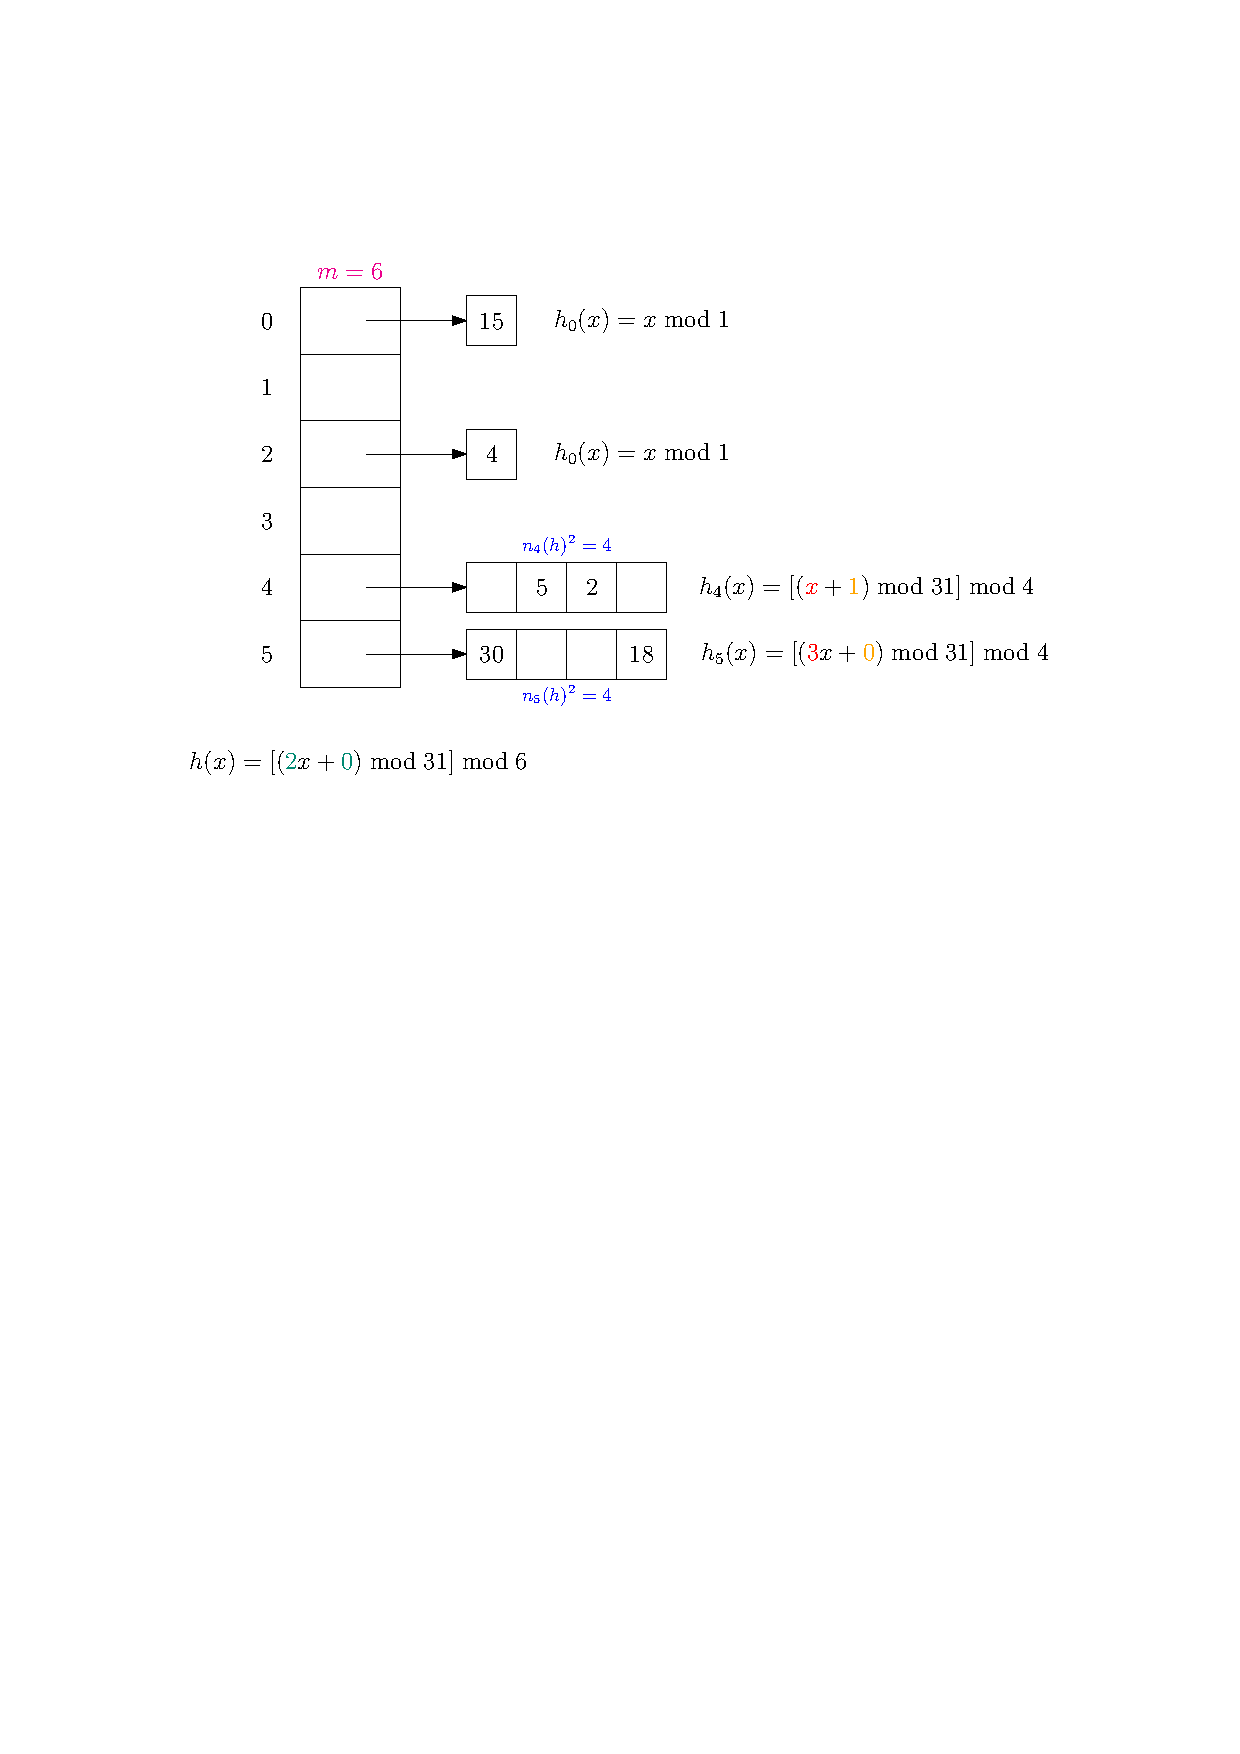
\includegraphics[width=0.6\linewidth]{fks-hashing-example.pdf}
        \caption{Example of a two-level hash table}
        \label{fig:fks-hashing-example}
    \end{figure}

    If we were to represent this two-level using a 1-D array, it should look like Figure \ref{fig:fks-hashing-example-array}
    \begin{figure}[htbp]
        \centering
        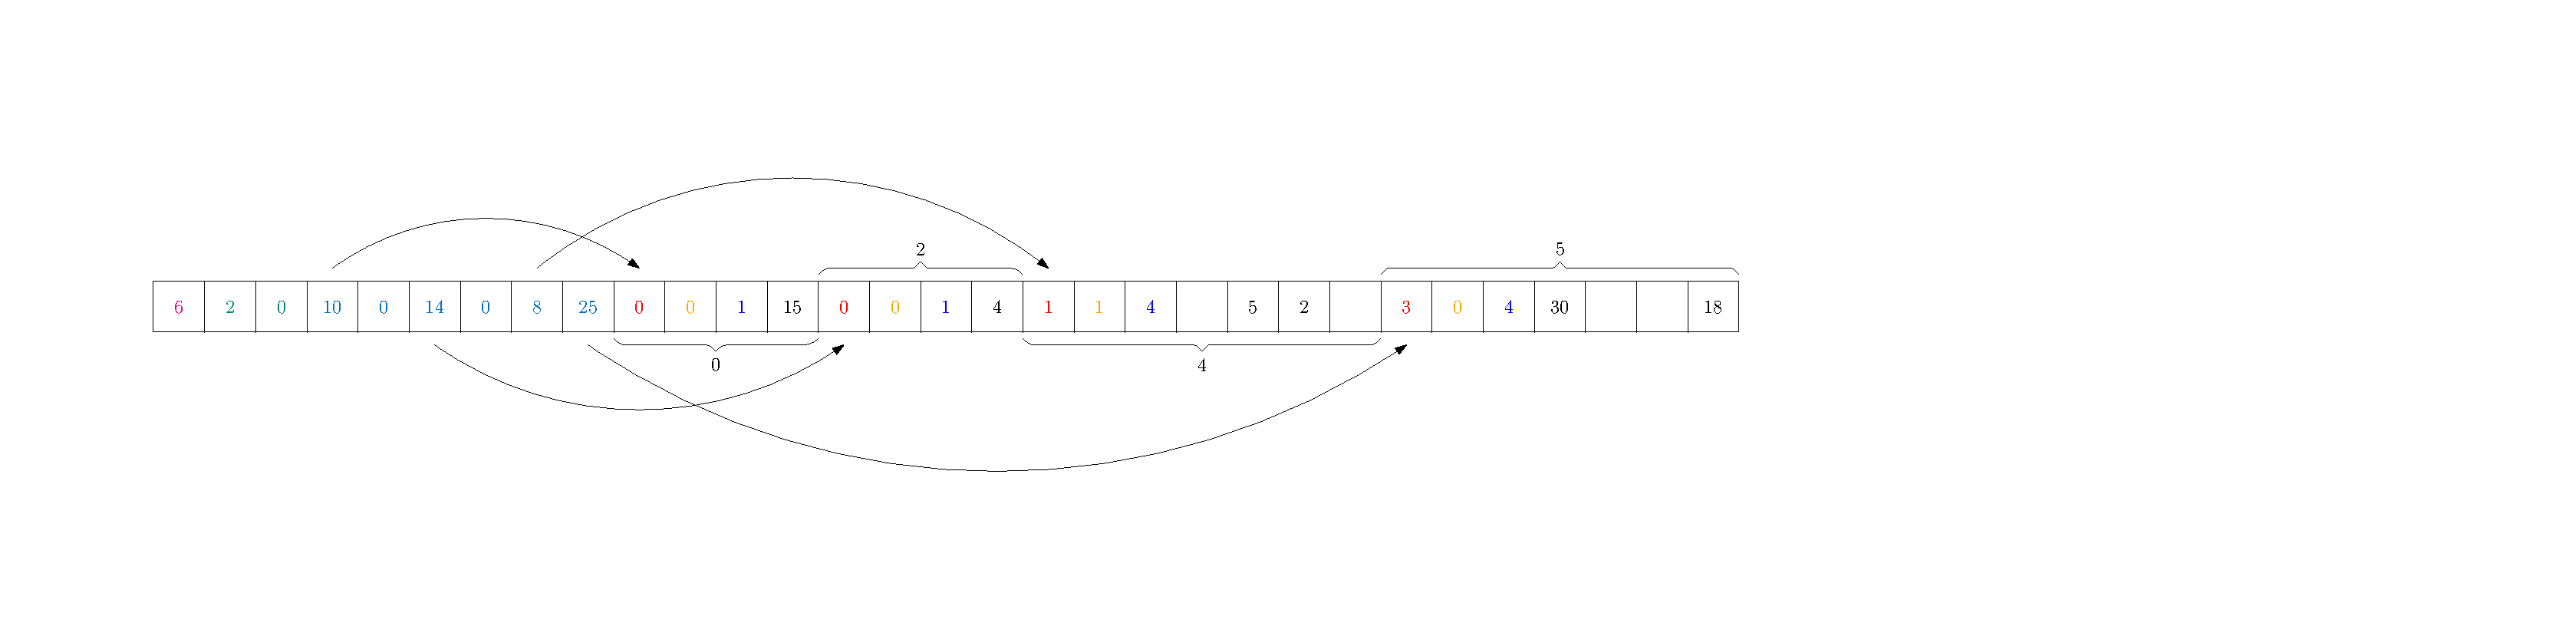
\includegraphics[width=\linewidth]{fks-hashing-example-array.pdf}
        \caption{The previous two-level hash table represented by an array. The colored represents the corresponding parameters in the two-level hash table representation.}
        \label{fig:fks-hashing-example-array}
    \end{figure}
\end{example}

\pagebreak

\begin{remark}
    This two-level hash table is often called the FKS hash table, which owes its name to its inventors M. Fredman, J. Koml\'{o}s, and E. Szemer\'{e}di. They published the article titled \href{https://www.cs.dartmouth.edu/~ac/Teach/CS105-Winter05/Handouts/fks-perfecthash.pdf}{\textit{Storing a Sparse Table with O(1) Worst Case Access Time}} in 1984, in which they first introduced this kind of hash table.
\end{remark}

\section{Application of Hashing}

Given an array $A$ of $n$ numbers, determine if all of them are different.

\begin{itemize}
    \item Sort the array and then check if adjacent numbers are duplicates. The time complexity would be $O(n\log n + n)$, where the $n\log n$ is from sorting the array and $n$ is for iterating over the array.
    \item Insert every element into the hash table on at a time. Each time, check for duplicates with a search. This take $\Theta(n)$ worst-case expected time.
\end{itemize}

Given a list of $n$ possible integers $x_1,x_2,\cdots,x_n$, determine in $O(n)$ worst-case expected time if there exists and $i$ and $j$ such that $x_i = x_j + 1$.

\chapter{Amortized Analysis}
\section{Amortized Cost}

\vspace{\parskip}

\begin{definition}[Worst-Case Sequence Complexity]
    The worst-case sequence complexity $C(m)$ is defined as
    $$
    C(m) = \max \{ T(\sigma) \mid \text{$\sigma$ is a sequence of $m$ operations} \}
    $$
    $C$ is a function of the length of the sequence.
\end{definition}

If there are many possible initial states, we use the notation $T(\sigma, S_0)$ and $C(m,S_0)$ where $S_0$ is an initial state.

To compute $C(m)$:

\begin{itemize}
    \item To get an upper bound on $C(m)$, prove that for every sequence $\sigma$ of $m$ operations, the time to process $\sigma$ from the initial initial state is $\leq f(m)$. Thus, $C(m) \leq f(m)$.
    \item To get a lower bound on $C(m)$, prove that for some sequence of $m$ operations from the initial state, the time to process $\sigma$ is $\geq g(m)$. Thus, $C(m) \geq g(m)$.
\end{itemize}

\begin{definition}[Amortized Cost] \index{amortized cost}
    The amortized cost per operation for a sequence of $n$ operations is the total cost of the operations divided by $n$. Formally,
    $$
    A(m) = \frac{C(m)}{m}
    $$
    for a sequence of $m$ operations.
\end{definition}

As an example, consider if you borrowed \$100k mortgage to buy a house. You need to pay it back over 10 years. Assume interest rate is 10\% per year.

There are two ways to pay the mortgage.

In general, the worst-case sequence complexity is less than or equal to $m$ times the worst-case complexity. This happens if every operation in that sequence is the worst case. It follows that the amortized complexity is always less than or equal to the worst-case complexity.

Example 1: sorted linked list. Sequence of $m$ insert and search operations starting from an empty list. For complexity measure, we count element comparison.

$i$th operation takes less than or equal to $i-1$ steps since before the $i$th operation, the list has length $\leq i-1$. So worst-case time for one operation in a sequence of $m$ operations is $m-1$.

For the amortized complexity, consider the sequence $\proc{Insert}(1), \, \proc{Insert}(2),\, \cdots \proc{Insert}(m)$. In this sequence, the $i$th operation performs exactly $i-1$ comparisons and
$$
T(\sigma) = \sum_{i=1}^m (i-1) = \frac{m(m-1)}{2}
$$
Thus the amortized complexity of insertions and searchings in a sorted linked list is at least $T(\sigma)/m = (m-1)/2$.

In this case, the worst-case complexity is a good upper bound for amortized complexity.

Example 2: increasing a binary counter starting from 0.

Consider an array $X$ $[0,\cdots,k-1]$ of bits representing an integer such that
$$
x = \sum_{i=0}^{k-1} X[i]\cdot 2^i.
$$
Initially, $x=0$.

We have an operation $\proc{Increment}(x)$ which adds 1 to $x$ modulo $2^k$.

The worst-case number of bit flips in an \proc{Increment} operation is $k$ (e.g. occurs when all bits of $X$ are 1).

There is only one sequence of $m$ \proc{Increment} operations. In this sequence, $X[0]$ is flipped $m$ times; $X[1]$ is flipped $\lfloor m/2 \rfloor$; $X[2]$ is flipped $\lfloor m/4 \rfloor$; and $X[i]$ is flipped $\lfloor m/2^i \rfloor$ times.

The worst-case sequence complexity is
$$
C(n) = \sum_{i=0}^{k-1} \left\lfloor \frac{m}{2^i} \right\rfloor < m \sum_{i=0}^\infty 2^{-i} = 2m
$$
Thus,
$$
A(m) = \frac{C(m)}{m} \leq 2
$$
while the worst-case complexity of an \proc{Increment} is $k$.

Generally, there are three methods for performing amortized analysis. Although all methods should give us the same answer, depending on the circumstances, some methods will be easier than others.

\begin{itemize}
    \item Aggregate analysis determines the upper bound $T(n)$ on the total cost of a sequence of $n$
    operations, then calculates the amortized cost to be $T(n) / n$.
    \item The accounting method determines the individual cost of each operation, combining its immediate execution time and its influence on the running time of future operations. We use the analogy of a bank account. Prior operations that may impact future operations can store some credits in the bank for uses by future operations. Usually, many short-running operations accumulate credits in small increments, while rare long-running operations use the credits.
    \item The potential method is like the accounting method, but the balance of the imaginary bank account at each state is given by the potential function.
\end{itemize}

\section{Aggregate Method}

Get an upper and lower bound on $C(m)$ worst-case sequence complexity and then divide it by $m$.

\section{Accounting Method}

Each kind of operation is assigned a fixed charge $a(\id{op})$ called the allocated charge or amortized cost of that operation.

When the allocated cost $a(\id{op})$ is greater than the actual cost of $\id{op}$, the excess is associated with specific objects in the data structure as credit.

Credit can be used later to help pay for operations where allocated costs are less than their actual costs. The can be viewed as storing money in a bank account for later uses.

If the total credit in the data structure is always non-negative (i.e. the bank account never runs out of money), then the total actual cost of the sequence of operations is less than or equal to the sum of allocated charges of the operations in the sequence.

To prove that the total credit in the data structure is always non-negative, we will use a credit invariant (similar to loop invariant used to prove correctness). The credit invariant is a rule that says that parts of the data structure with certain properties will have a certain number of credits associated with them. Credit invariants are proved by induction.

Sometimes, credits are needed to establish the credit invariant for the initial state. The total actual cost of the sequence is less than or equal to the cost to establish the credit invariant plus the sum of allocated charge to the operations in the sequence.

\begin{remark}
    It is important not to explicitly implement the credit system in the code. It is for analysis purpose only.
\end{remark}

The initial value of the account is 0. We define that \$1 is the cost of one bit flip.

The allocated charge to \proc{Increment} is \$2.

The credit invariant is: Each bit with value value 1 has \$1 credit.

When we flip a bit from 0 to 1, we use \$1 to actually flip that bit, and store the additional \$1 as the credit on that bit (in order to maintain the credit invariant).

When we flip a bit from 1 to 0, the associated \$1 credit at that bit can be used to pay for performing the bit fip.

\begin{proof}
    Initially, all bits are 0, so the credit invariant is vacuously true.

    Assume that the credit invariant is true before an \proc{Increment} operation. Then, all bits of 1 in $X$ contain a \$1 credit.

    Case 1: the $i$ least significant bits $X[0],\cdots,X[i-1]$ are 1, and $X[i] = 0$ for some $i$ such that $0 \leq i \leq k$. The actual number of bit flips in this case is $i+1$. Use the $i$ credits associated with the $i$ least significant bits to pay for flipping these bits from 1 to 0. Use \$1 of allocated charge to pay for flipping $X[i]$ from 0 to 1. Use the remaining \$1 of allocated charge to associate as credit with $X[i]$. All other 1 bits still have \$1 credit. Thus the credit invariant is true after this \proc{Increment} operation.

    Case 2: all of the bits are 1. All $k$ bits are flippted, use the $k$ credits on these bits to pay for the flips. This maintains the credit invariant. The allocated charge can be donated to charity (LOL).

    Then by induction, the credit invariant is true after every \proc{Increment} operation. The cost to establish the credit invariant is 0.

    The total actual cost of $m$ operations $C(m) \leq 0 + 2m$. Hence, the amortized cost $A(m)$ of \proc{Incremente} is at most 2 bit flips.  
\end{proof}

\section{Dynamic Array}

In this section, we will consider the data structure known as dynamic array. It is similar to a regular array, but its length changes according to the ``fullness'' of the array.

\index{dynamic array}

The array will be initialized with a fixed length. Upon calling \textsc{Insert}, it will insert an element into the array, and whenver the current array becomes full, we create a longer array and copy everything into the new array. Similarly, after calling \textsc{Delete}, we will shrink the array whenever the array becomes too empty. If we only consider the worst case, the runtime complexities are bad: $O(n)$ for both operations. However, if we look at the amortized cost, the runtime is actually smaller.

\begin{figure}[htbp]
    \captionsetup{singlelinecheck=false, font=footnotesize, labelsep=space, margin={0pt,1cm}, justification=raggedright}
    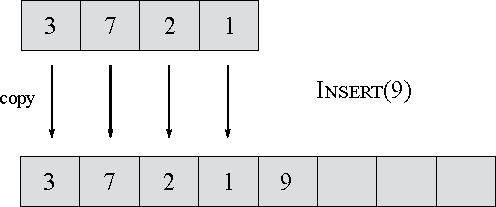
\includegraphics[width=0.4\linewidth]{figures/dynamic_arr_append.pdf}

    \hfill

    \caption[width=0.5\linewidth]{The dynamic array after the operation \textsc{Insert}(9). The length of the new array is doubled, and old elements are copied to the new array.}
\end{figure}

\subsection{Accounting Method Analysis for Dynamic Array}

\begin{figure}[htbp]
    \centering
    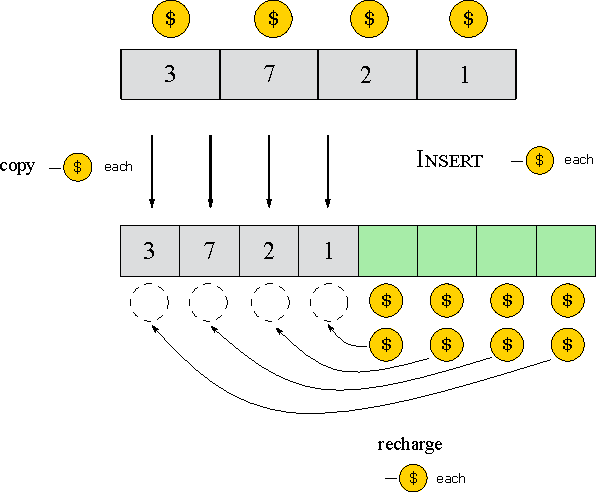
\includegraphics[width=0.6\linewidth]{figures/accounting_method_insert.pdf}
    \caption{<caption>}
\end{figure}

\section{Potential Method}

\vspace{\parskip}

Prepaid wors in represented as potential energy associated with the whole data structure. Potential energy in a data structure can be released to pay for later operations.

\begin{definition}[Potential Function] \index{potential function}
    Let $D$ be some data structure with initial state $D_0$. For each $i = 1,2,\cdots,n$, let $c_i$ be the actual cost of the $i$-th operation and $D_i$ be the resulting data structure after applying the $i$-th operation to data structure $D_{i-1}$.

    The potential function $\Phi$ maps each data structure at state $i$, denoted $D_i$, to a real number $\Phi(D_i)$, which is the potential associated with data structure $D_i$.

    The amortized cost $\hat{c_i}$ of the $i$-th operation with respect to the potential function $\Phi$ is
    $$
    \hat{c_i} = c_i + \Phi(D_i) - \Phi(D_{i-1})
    $$
    And the total amortized cost of $n$ operations is
    $$
    \sum_{i=1}^{n} \hat{c_i} = \sum_{i=1}^{n} \left( c_i + \Phi(D_i) - \Phi(D_{i-1}) \right) = \sum_{i=1}^{n} c_i + \Phi(D_n) - \Phi(D_0)
    $$
\end{definition}

\subsection{Analysis of Binary Counter Using Potential Method}

Let $C_i$ be the configuration after $i$th \proc{Increment}.

Let $\Phi(c)$ be the number of 1 bits in the stored representation of the counter in counfiguration $C$.

$\Phi(C) \geq 0$ for all configurations $C$. $\Phi(C) = 0$ since all bits are 0 initially.


\part{Advanced Data Structures}

\chapter{Dynamic Arrays}

\chapter{Fibonacci Heaps}

\chapter{Disjoint Sets}


\part{Lower Bounds}

\chapter{Decision Trees}
\section{Lower Bounds} \index{lower bound} \index{model of computation} \index{comparison model}

So far, we have been talking almost exclusively about how we can use different algorithms and data structures to solve certain problems as fast as possible. In this part, we will focus on proving certain problems cannot be solved as quickly as we might want. In other words, there is a limit to how good we can do. For example, in a comparison model, sorting can only be achieved at best in $\Omega(n \log n)$ time in the worst case.

\begin{definition}
    Let $P$ be a problem. The worst case complexity of problem $P$ is
    $$
    C(P) = \min \{ C_A \mid \text{$A$ is an algorithm that solves $P$} \}
    $$
    where $C_A:\; \N \to \N$ is the worst case complexity of algorithm $A$.
\end{definition}

We can prove the upper-bound of the complexity of a problem by giving a specific algorithm $A$ that solves $\Pi$, and faster algorithms give us smaller (tighter and better) upper bounds.

However, to prove that a problem has a certain lower bound, it is not enough to give an algorithm and say that we cannot do better. We have to show that every algorithm that solves $\Pi$ has a worst-case running time $\Omega(f(n))$, or equivalently, that there is no algorithm that solves $\Pi$ that runs in $o(f(n))$ time. To be more specific, we need to specify what kinds of algorithms we want to consider, which is formally known as model of computation. For example, the comparison model is one model that is used to solve sorting and searching problems.


Let $\mathcal{A}$ be a class of algorithms. The worst-case complexity of problem $P$ in class $\mathcal{A}$ is
$$
C(P) = \min \{ C_A \mid \text{$A \in \mathcal{A}$ is an algorithm that solves $P$} \}
$$
$\mathcal{A} \subseteq \mathcal{A}'$ implies that a lower bound on the worst-case complexity of $P$ in class $\mathcal{A}'$ is also a lower bound on the worst-case complexity of $P$ in class $\mathcal{A}$. In other words, lower bounds in more powerful models are better.

\section{Comparison Model}

In the comparison model, we consider all input items as black boxes, or more precisely, ADTs. The only operations allowed on the items are comparisons: $<, \leq, >, \geq, =$. Most searching and sorting algorithms we have been looking at so far use the comparison model: heap sort, merge sort, binary search and binary search tree, etc. In the comparison model, we count the number of comparisons and define it as the time cost of the algorithm.

\section{Comparison Tree}

\subsection{Intuition}

Any comparison algorithm can be viewed as a tree of all possible comparisons, the outcomes of the comparisons, and the resulting answer. This tree is called a decision tree. There is a different tree for each different input size.

For any particular $n$,
\begin{itemize}
    \item \textit{internal node} corresponds to a decision in the algorithm (in this case, comparisons)
    \item \textit{edge} corresponds to a possible outcome of the comparison denoted by the node
    \item \textit{leaf} corresponds to a possible answer (output) of the problem
    \item \textit{root-to-leaf path} corresponds to an execution of the algorithm
    \item \textit{length of the root-to-leaf path} corresponds to the time cost of the execution associated with that path
    \item \textit{height of the tree} (or depth of the deepest leaf) corresponds to the worst-case running time.
\end{itemize}


\subsection{Decision Tree for Searching}

Consider a comparison tree for the binary search algorithm. An example is shown below for binary search for $x$ in $A[1\ldots 3]$ using only $\leq$ comparisons and outputs $i$ such that $x=A[i]$ or 0 if no such element exists.

The average case complexity the algorithm is the expected path length, that is the weighted average depths of the leaves.
$$
\sum_{\ell} (\attrib{\ell}{depth}) \cdot \Prob [\text{input leads to $\ell$}]
$$

Another example is for searching in $[2,3,5,7,11,13,17,19]$ using $<$ and $=$ comparisons. 

\hfill

\begin{figure}[htbp]
    \centering
    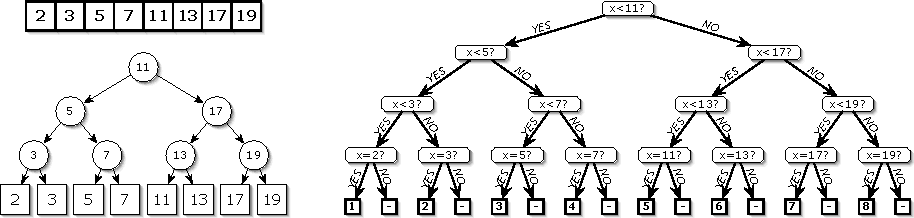
\includegraphics[width=\linewidth]{figures/binary_search_decision_tree.pdf}
    \caption{Decision tree for searching the array containing $[2,3,5,7,9,11,13,17,19]$.}
    \label{fig:sorting-tree-2}
\end{figure}

\subsection{Decision Tree for Sorting}

\chapter{Information Theory}

\chapter{Adversary Arguments}

\chapter{Reduction}


\part{Graphs}

\chapter{Breadth-First Search}
\section{Definition}

\vspace{\parskip}

\begin{definition}[Graphs] \index{graphs} \index{vertices} \index{edges}
    A graph is defined as a tuple $G=(V,E)$ where $V$is an arbitrary non-empty finite set, whose elements are called vertices or nodes; and $E$ is a set of pairs of elements of $V$, which we call edges. For an undirected graph, the edges are unordered pairs ${u,v}$. In a directed graph, the edges are ordered pairs $(u,v)$.
\end{definition}

\begin{definition}[Neighbors and Degrees] \index{neighbors} \index{predecessor} \index{successor} \index{degree} \index{in-degree} \index{out-degree}
    For any edge $uv$ in an undirected graph, we call $u$ neighbor of $v$ and vice versa, and we say that $u$ and $v$ are adjacent. The degree of a node is its number of neighbors.

    In directed graphs, for every edge $u \to v$, we call $u$ a predecessor of $v$, and we call $v$ a successor of $u$. The in-degree of a vertex is its number of predecessors; the out-degree is its number of sucessors.
\end{definition}

\begin{definition}[Subgraphs] \index{subgraphs}
    A graph $G' = (V',E')$ is a subgraph of $G=(V,E)$ if $V' \subseteq V$ and $E' \subseteq E$. A proper subgraph of $G$ is any subgraph that is not $G$ itself.
\end{definition}

\section{Representations of Graphs}

\subsection{Adjacency List}

\vspace{\parskip}

\begin{definition}[Adjacency List] \index{adjacency-list}
    The adjacency-list representation of a graph $G=(V,E)$ consists of an arrray \textit{Adj} of $|V|$ lists, one for each vertex in $V$. For each $u \in V$, the adjacency list \textit{Adj[u]} contains all the vertices $v$ such that there is an edge $(u,v) \in E$. That is, \textit{Adj}[u] contains all the vertices adjacent to $u$ in $G$.
\end{definition}

\section{Breadth-first Search} \index{breadth-first search (BFS)}

Given a graph $G=(V,E)$ and a distinguished source vertex $s$, breadth-first search systematically explores the edges of $G$ to discover every vertex that is reachable from $s$. Breadth-first search expands the frontier between disvoered and undiscovered vertices uniformly across the breadth of the frontier. The algorithm discovers all vertices at distance $k$ from $s$ before discovering any vertices at distance $k+1$.

BFS visits all the vertices in a connected undirected graph in order of their distance from the start vertex $s$. As we visit the nodes, we can also determine $\delta(s,v)$ which is the distance from $s$ to $v$, that is, the number of edges on the shortest path from $s$ to $v$.

\begin{codebox}
    \Procname{$\proc{BFS}(s)$}
    \li $Q = \proc{Queue}(\{\})$;\; $d = [ \, ]$ 
    \li \For $v \in V$ \Do
        \li $d[v] = 0$ 
        \li label $v$ as unvisited \End
    \li visit $s$
    \li $\color{cyan} \pi[s] = \const{nil}$ 
    \li $\proc{Enqueue}(Q,s)$
    \li \While $Q \neq \emptyset$ \Do
        \li $u = \proc{Head}(Q)$
        \li \For {\color{cyan}out} neighbor $v$ of $u$ \Do
            \li \If $v$ is unvisited \Then
                \li $\proc{Enqueue}(Q,v)$
                \li $d[v] = d[u] + 1$
                \li \color{cyan} $\pi[v] = u$  \End
            \End
        \li $\proc{Dequeue}(Q)$
\end{codebox}

We keep track of the shortest length from $s$ to each vertex in the array $d$.

If $G$ is not connected, this algorithm visits the connected component of $G$ containing $s$. If $G$ is directed, this visits all vertices reachable from $s$ by a directed path.

\textit{Claim}. If $G$ is connected, then at the end of BFS, $d[v] = \delta(s,v)$ for all $v \in V$.

Tree edge: $\{v,\, \attrib{v}{parent}\}$ or $(\attrib{v}{parent},\, v)$ if directed.

Cross edge: $\{ u,v \}$ or $(u,v)$ if directed where $u$ is not an ancestor of descendant of $v$ in the BFS tree.

Back edge: edge from a node to one of its ancestors.

\begin{lemma}
    If $G$ is undirected, then all edges are tree edges or cross edges.
\end{lemma}

\begin{proof}
    Suppose that $\{u,v\}$ is a back edge discovered when $u$ is at the head of $Q$.

    Since $v$ is an ancestor of $u$, it was visited and hence enqueued before $u$. So $v$ was the head of $Q$ before $u$. Since $\{u,v\} \in E$, $u$ was visited when $v$ was at the head of $Q$.This means that $\{u,v\}$ is a tree edge.
\end{proof}

If represented using an adjacency list, the BFS algorithm is $O(n+m)$. Each node $v$ is enqueued at most once. Its adjacency list is examined at most once. If represnted using an adjacency matrix, it requires $\Theta(n^2)$ time.

$d[v]=0$ if and only if $v=s$. If $G$ is directed, $(\pi[v],\, v) \in E$. If $G$ is undirected, $\{ \pi[v], v \} \in E$. $d[v] = d[\pi[v]]+1$.

\begin{lemma}
    At the end of the BFS, $d[v] \geq \delta(s,v)$ for all nodes reachable from $s$.
\end{lemma}

\begin{proof}
    $d[v]$ is the length of the path from $s$ to $v$ in the BFS tre since $d[v] = d[\pi[v]] + 1$ for all nodes $v \neq s$ reachable from $s$.

    All these edges are in $E$, so $\delta(s,v) \leq d[v]$.
\end{proof}

\begin{lemma}
    Let $s=v_1,v_2,\cdots,v_n$ be the nodes in the order they are visited (enqueued). Then, $0=d[v_1] \leq \cdots \leq d[v_n]$. 
\end{lemma}

\begin{proof}
    Suppose not. Let $j>1$ be the smallest integer such that $d[v_j]<d[v_{j-1}]$.
    
    Let $v_h = \pi[v_{j-1}]$ where $h < j-1$, and let $v_i = \pi[v_j]$ where $i < j$.
    
    $d[v_{j-1}] = 1 + d[v_{h}]$ and $d[v_j] = 1 + d[v_i]$. Since $d[v_{j-1}] > d[v_j]$, then $d[v_h] > d[v_i]$. This implies that $i<h$. So, $d[v_j] \leq d[v_i]$ and $d[v_h] \leq d[v_{j-1}]$.

    This means $v_i$ is enqueued and hence dequeued before $v_h$, which then implies that $v_j$ was enqueued before $v_{j-1}$. This is a contradiction.
\end{proof}

\begin{theorem}
    At the end of $\proc{BFS}(s)$, $d[v] = \delta(s,v)$ for all nodes $v$ reachable from $s$.
\end{theorem}

\begin{proof}
    Consider the shortest path (of length) $\delta(s,v)$ from $s$ to $v$ in $G$. Let $\{u,v\}$ be the last edge in this path. $\delta(s,u) = \delta(s,v) - 1$.

    $\delta(s,s) = 0 = d[s]$. Let $v$ be a vertex where this is not ture. That is, let $v$ be a vertex with minimum value of $\delta(s,v)$ such that $d[v] < \delta(s,v)$. In particular, we know that $\delta(s,u) = d[u]$ and $\delta(s,v) = d[v] = d[\pi[v]]+1$. So, $d[v] > d[u] + 1$. This implies that $u$ is enqueued before $\pi[v]$. This is a contradiction, so no such $v$ exists.
\end{proof}


\chapter{Depth-First Search}

\chapter{Minimum Spanning Trees}

\chapter{Bellman-Ford's Algorithm}

\chapter{Dijkstra's Algorithm}




%----------------------------------------------------------------------------------------
%	APPENDIX
%----------------------------------------------------------------------------------------

\part*{Appendix}
\appendix
\chapter*{Commonly Used Axioms \& Theorems}
\addcontentsline{toc}{chapter}{\textcolor{ocre}{Axioms \& Theorems}} 
\section*{Rules of Inference} \label{rulesofinference}

\begin{axiom_appendix}[Modus Ponens]
$(P \wedge (P \implies Q)) \implies Q $
\end{axiom_appendix}

\begin{axiom_appendix}[Modus Tollens]
$(\neg Q \wedge (P \implies Q)) \implies \neg P $
\end{axiom_appendix}

\begin{axiom_appendix}[Hypothetical Syllogism (transitivity)]
\hfill

$((P \implies Q) \wedge (Q \implies R)) \implies (P \implies R) $
\end{axiom_appendix}

\begin{axiom_appendix}[Disjunctive Syllogism]
$((P \vee Q) \wedge \neg P) \implies Q$
\end{axiom_appendix}

\begin{axiom_appendix}[Addition]
$P \implies (P \vee Q)$
\end{axiom_appendix}

\begin{axiom_appendix}[Simplification]
$(P \wedge Q) \implies P$
\end{axiom_appendix}

\begin{axiom_appendix}[Conjunction]
$((P) \wedge (Q)) \implies (P \wedge Q)$
\end{axiom_appendix}

\begin{axiom_appendix}[Resolution]
$((P \vee Q) \wedge (\neg P \vee R)) \implies (Q \vee R)$
\end{axiom_appendix}

\section*{Laws of Logic}

\begin{axiom_appendix}[Implication Law]
$(P \implies Q) \equiv (\neg P \vee Q)$
\end{axiom_appendix}

\begin{axiom_appendix}[Distributive Law]
\begin{align*}
    (P \wedge (Q \vee R)) &\equiv ((P \wedge Q) \vee (P \wedge R)) \\
    (P \vee (Q \wedge R)) &\equiv ((P \vee Q) \wedge (P \vee R))
\end{align*}
\end{axiom_appendix}

\begin{axiom_appendix}[De Morgan's Law]
\begin{align*}
    \neg (P \wedge Q) &\equiv (\neg P \vee \neg Q) \\
    \neg (P \vee Q) &\equiv (\neg P \wedge \neg Q)
\end{align*}
\end{axiom_appendix}

\begin{axiom_appendix}[Absorption Law]
\begin{align*}
    (P \vee (P \wedge Q)) &\equiv P \\
    (P \wedge (P \vee Q)) &\equiv P
\end{align*}
\end{axiom_appendix}

\begin{axiom_appendix}[Commutativity of AND]
$A \wedge B \equiv B \wedge A$
\end{axiom_appendix}

\begin{axiom_appendix}[Associativity of AND]
$(A \wedge B) \wedge C \equiv A \wedge (B \wedge C)$
\end{axiom_appendix}

\begin{axiom_appendix}[Identity of AND]
$\textbf{T} \wedge A \equiv A$
\end{axiom_appendix}

\begin{axiom_appendix}[Zero of AND]
$\textbf{F} \wedge A \equiv \textbf{F}$
\end{axiom_appendix}

\begin{axiom_appendix}[Idempotence for AND]
$A \wedge A \equiv A$
\end{axiom_appendix}

\begin{axiom_appendix}[Contradiction for AND]
$A \wedge \neg A \equiv \textbf{F}$
\end{axiom_appendix}

\begin{axiom_appendix}[Double Negation]
$\neg (\neg A) \equiv A$
\end{axiom_appendix}

\begin{axiom_appendix}[Validity for OR]
$A \vee \neg A \equiv \textbf{T}$
\end{axiom_appendix}

\section*{Induction}
\begin{axiom_appendix}[Well Ordering Principle]
Every nonempty set of nonnegative integers has a smallest element. i.e., For any $A \subset \N$ such that $A \neq \emptyset$, there is some $a \in A$ such that $\forall a' \in A.a\leq a'$.
\end{axiom_appendix}

\chapter*{Basic Prerequisite Mathematics}
\addcontentsline{toc}{chapter}{\textcolor{ocre}{Basic Prerequisite Mathematics}}
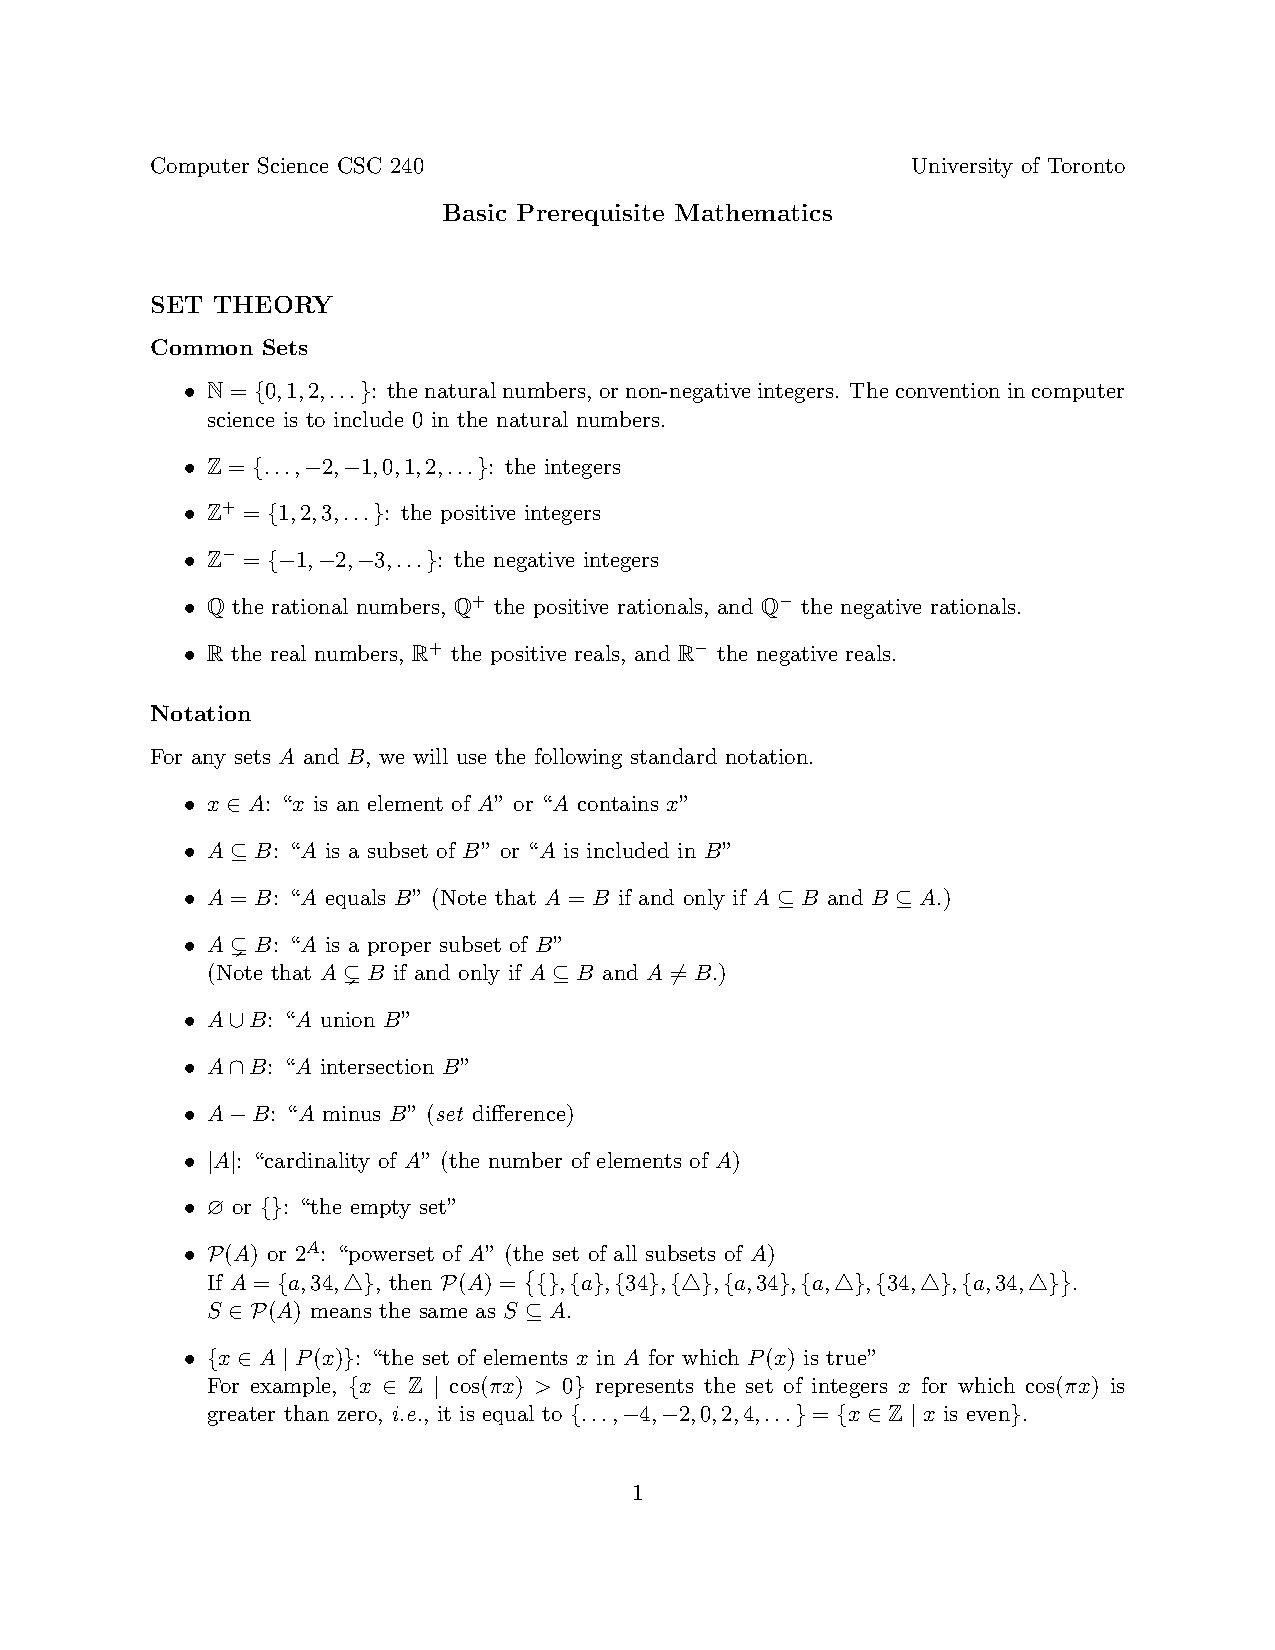
\includepdf[pages=-]{appendix/basicMath.pdf}

\chapter*{Proof Templates}
\addcontentsline{toc}{chapter}{\textcolor{ocre}{Proof Templates}}
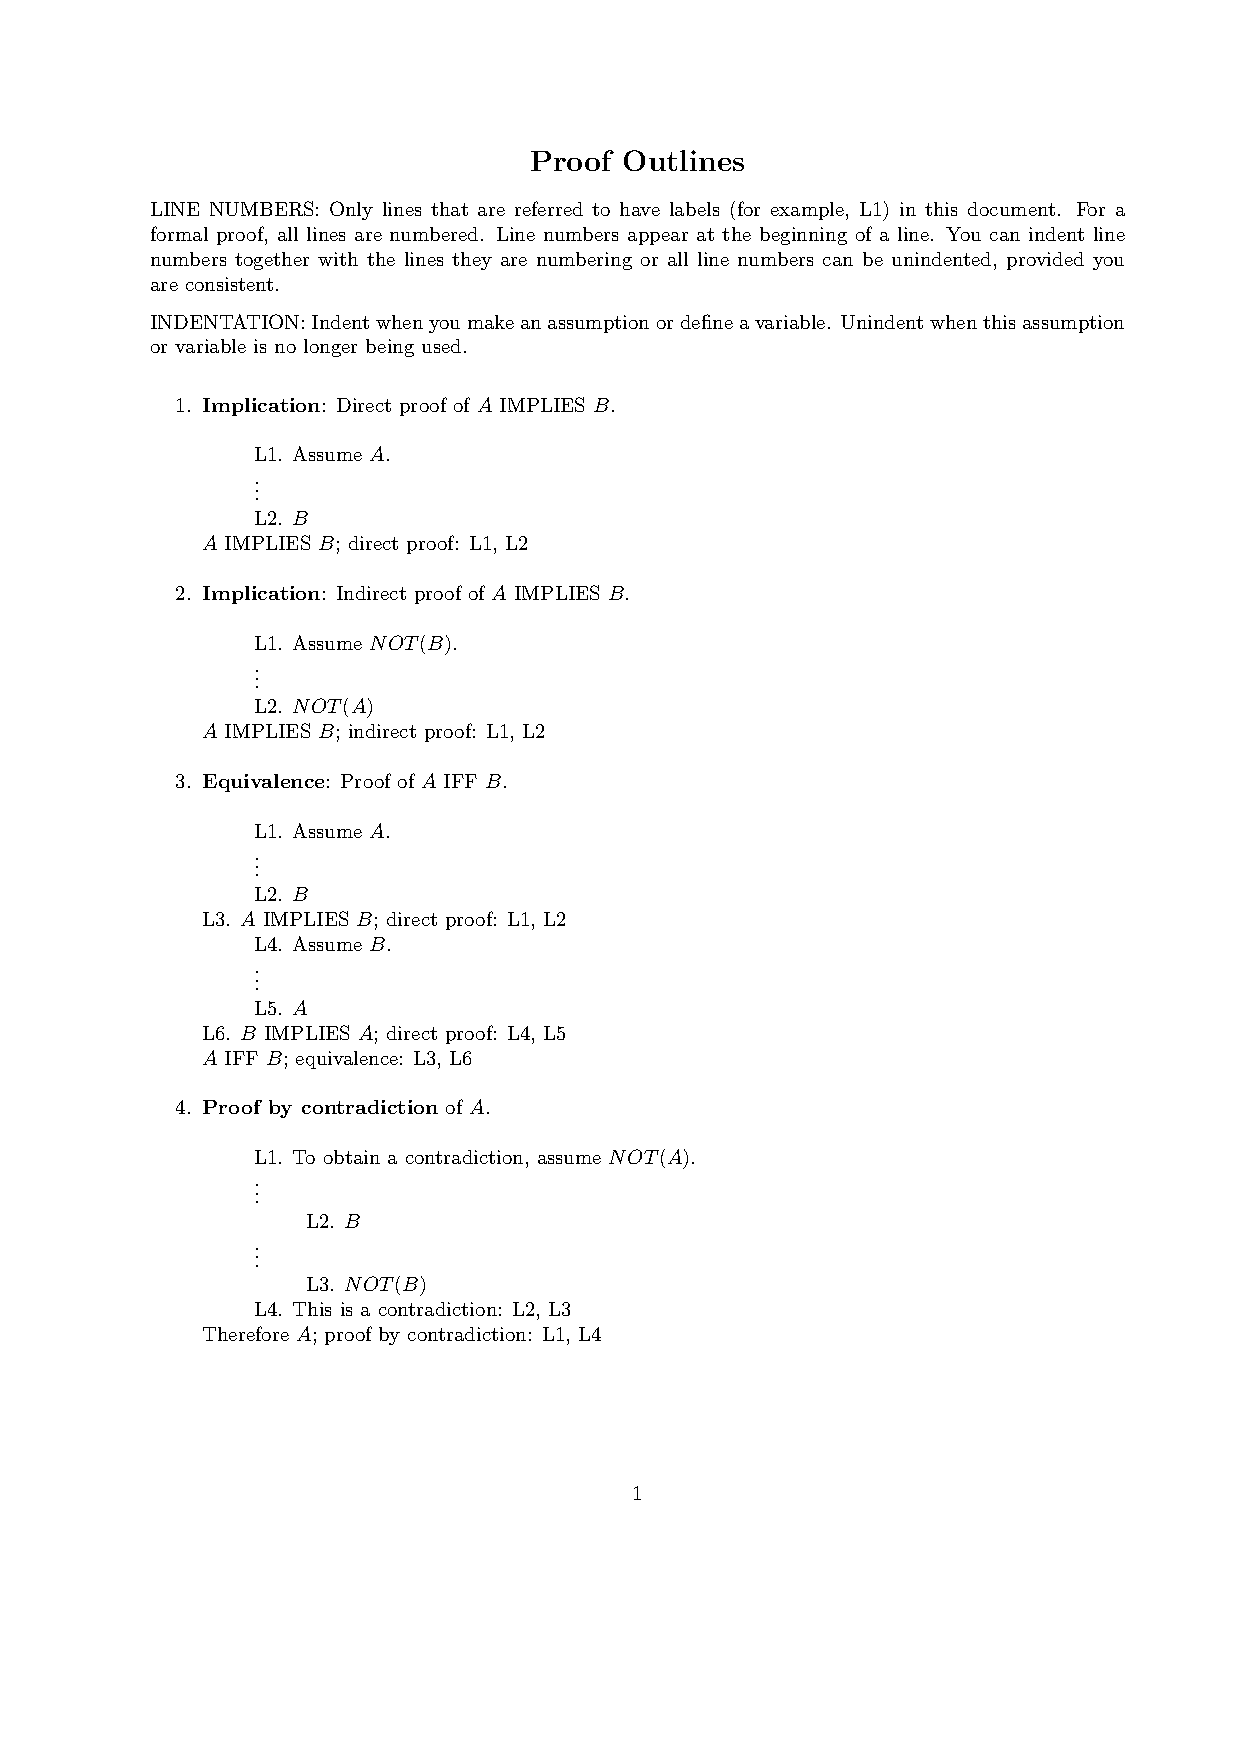
\includepdf[pages=-]{appendix/proofOutlines.pdf}

%----------------------------------------------------------------------------------------
%	INDEX
%----------------------------------------------------------------------------------------

\chapter*{Index}

\cleardoublepage % Make sure the index starts on an odd (right side) page
\phantomsection
\setlength{\columnsep}{0.75cm} % Space between the 2 columns of the index
\addcontentsline{toc}{chapter}{\textcolor{ocre}{Index}} % Add an Index heading to the table of contents

\printindex % Output the index

%------------------------------------------------
%   BIBLIOGRAPHY ENTRIES
%------------------------------------------------
\chapter*{Bibliography}
\addcontentsline{toc}{chapter}{\textcolor{ocre}{Bibliography}} % Add a Bibliography heading to the table of contents

\section*{Courses}
\addcontentsline{toc}{section}{Courses}
\printbibliography[heading=bibempty,type=misc]

\section*{Books}
\addcontentsline{toc}{section}{Books}
\printbibliography[heading=bibempty,type=book]

\newpage

%------------------------------------------------
%   TUTORIALS
%------------------------------------------------
\definecolor{ocre}{HTML}{4c9d4c}
\part*{Tutorial}

\newpage

%----------------------------------------------------------------------------------------

\end{document}
